\documentclass{book}

\usepackage{amsthm,pat}

% This allows the use of \verb inside footnotes
\usepackage{fancyvrb}
\VerbatimFootnotes

\usepackage{listings}
\usepackage[usenames,dvipsnames]{color}

\setlength{\textheight}{8.5in}
\setlength{\textwidth}{6in}
\setlength{\topmargin}{-0.375in}
\setlength{\oddsidemargin}{.25in}
\setlength{\evensidemargin}{.25in}
\setlength{\headheight}{0.200in}
\setlength{\headsep}{0.4in}
\setlength{\footskip}{0.500in}
\setlength{\parskip}{1ex}
\setlength{\parindent}{1.25cm}
\flushbottom

\lstset{
  language=java,
  basicstyle=\small\ttfamily,
  keywordstyle=\color{RoyalPurple},
  identifierstyle=\color{Blue},
  stringstyle=\color{Blue},
  showstringspaces=false,
  commentstyle=\color{ForestGreen},
  tabsize=2,
  frame=single
}


\title{Basic Data Structures (in Java)}
\author{Pat Morin}

\pagenumbering{roman}


\begin{document}
\begin{titlepage}
\maketitle
\thispagestyle{empty}
\end{titlepage}

\tableofcontents

\chapter{Array-Based Lists and Queues}
\chaplabel{arrays}

In this chapter, we study implementations of the \mbox{\texttt{List}} and \mbox{\texttt{Queue}}
interfaces where the underlying data is stored in an array, called the
\emph{backing array}.  The following table summarizes the running times
of operations for the data structures presented in this chapter:

\noindent
\begin{tabular}{lcccc}
 & \mbox{\texttt{get({\color{var}i})}} & \mbox{\texttt{set({\color{var}i},{\color{var}x})}} & \mbox{\texttt{add({\color{var}i},{\color{var}x})}} & \mbox{\texttt{remove({\color{var}i})}} \\
\mbox{\texttt{ArrayStack}} & $O(1)$ & $O(1)$ & $O(1+\mbox{\texttt{{\color{var}n}}}-\mbox{\texttt{{\color{var}i}}})$ & $O(\mbox{\texttt{{\color{var}n}}}-\mbox{\texttt{{\color{var}i}}})$ \\
\mbox{\texttt{ArrayDeque}} & $O(1)$ & $O(1)$ & $O(1+\min\{\mbox{\texttt{{\color{var}i}}},\mbox{\texttt{{\color{var}n}}}-\mbox{\texttt{{\color{var}i}}}\})$ 
             & $O(1+\min\{\mbox{\texttt{{\color{var}i}}},\mbox{\texttt{{\color{var}n}}}-\mbox{\texttt{{\color{var}i}}}\})$ \\
\mbox{\texttt{DualArrayDeque}} & $O(1)$ & $O(1)$ & $O(1+\min\{\mbox{\texttt{{\color{var}i}}},\mbox{\texttt{{\color{var}n}}}-\mbox{\texttt{{\color{var}i}}}\})$ 
             & $O(1+\min\{\mbox{\texttt{{\color{var}i}}},\mbox{\texttt{{\color{var}n}}}-\mbox{\texttt{{\color{var}i}}}\})$ \\
\mbox{\texttt{RootishArrayStack}} & $O(1)$ & $O(1)$ & $O(1+\mbox{\texttt{{\color{var}n}}}-\mbox{\texttt{{\color{var}i}}})$ & $O(\mbox{\texttt{{\color{var}n}}}-\mbox{\texttt{{\color{var}i}}})$ \\
\end{tabular}

Data structures that work by storing data in a single array have many
advantages and limitations in common:
\begin{itemize}
  \item Arrays offer constant time access to any value in the array.
  This is what allows \mbox{\texttt{get({\color{var}i})}} and \mbox{\texttt{set({\color{var}i},{\color{var}x})}} to run in constant time.
  \item Arrays are not very dynamic.  Adding or removing an element
  near the middle of a list means that a large number of elements in the
  array need to be shifted to make room for the newly added element or
  to fill in the gap created by the deleted element.  This is why the operations
  \mbox{\texttt{add({\color{var}i},{\color{var}x})}} and \mbox{\texttt{remove({\color{var}i})}} have running times that depend on \mbox{\texttt{{\color{var}n}}} and \mbox{\texttt{{\color{var}i}}}.
  \item Arrays can not expand or shrink.  When the number of elements in
  the data structure exceeds the size of the backing array, a new array needs
  to be allocated and the data from the old array needs to be copied
  into the new array.  This is an expensive operation.
\end{itemize}
The third point is important.  The running times cited in the table
above do not include the cost of growing and shrinking the backing array.
We will see that, if carefully managed, the cost of growing and shrinking
the backing array does not add much to the cost of an \emph{average}
operation.  More precisely, if we start with an empty data structure,
and perform any sequence of $m$ \mbox{\texttt{add({\color{var}i},{\color{var}x})}} or \mbox{\texttt{remove({\color{var}i})}} operations,
then the total cost of growing and shrinking the backing array, over the
entire sequence of $m$ operations is $O(m)$.  Although some individual
operations require growing or shrinking the backing array, and are
therefore expensive, the amortized cost, when amortized over all $m$
operations is only $O(1)$ per operation.

\section{\mbox{\texttt{ArrayStack}}: Fast Stack Operations Using an Array}
\seclabel{arraystack}
% TODO: One big figure showing add(x), remove() and resize()
An \mbox{\texttt{ArrayStack}} implements the list interface using an array \mbox{\texttt{{\color{var}a}}}, called
the \emph{backing array}.  The list element with index \mbox{\texttt{{\color{var}i}}} is stored
in \mbox{\texttt{{\color{var}a}[{\color{var}i}]}}.  At most times, \mbox{\texttt{{\color{var}a}}} is larger than strictly necessary,
so an integer \mbox{\texttt{{\color{var}n}}} is used to keep track of the number of elements
actually stored in \mbox{\texttt{{\color{var}a}}}.  In this way, the list elements are stored in
\mbox{\texttt{{\color{var}a}[0]}},\ldots,\mbox{\texttt{{\color{var}a}[{\color{var}n}-1]}} and, at all times, $\mbox{\texttt{{\color{var}a}.{\color{var}length}}} \ge \mbox{\texttt{{\color{var}n}}}$.

\begin{Verbatim}[tabsize=2,frame=single,commandchars=\\@\$,label=\texttt{ArrayStack},labelposition=topline]
	@\color@keyword$T$[] @\color@var$a$;
	@\color@keyword$int$ @\color@var$n$;
	@\color@keyword$int$ size() {
		@\color@var$return$ @\color@var$n$;
	}
\end{Verbatim}

\subsection{The Basics}

Accessing and modifying the elements of an \mbox{\texttt{ArrayStack}} using \mbox{\texttt{get({\color{var}i})}}
and \mbox{\texttt{set({\color{var}i},{\color{var}x})}} is trivial. After performing any necessary bounds-checking
we simply return or set, respectively, \mbox{\texttt{{\color{var}a}[{\color{var}i}]}}.

\begin{Verbatim}[tabsize=2,frame=single,commandchars=\\@\$,label=\texttt{ArrayStack},labelposition=topline]
	@\color@keyword$T$ get(@\color@keyword$int$ @\color@var$i$) {
		@\color@keyword$if$ (@\color@var$i$ < 0 || @\color@var$i$ > @\color@var$n$ - 1) @\color@keyword$throw$ @\color@keyword$new$ IndexOutOfBoundsException();
		@\color@var$return$ @\color@var$a$[@\color@var$i$];
	}
	@\color@keyword$T$ set(@\color@keyword$int$ @\color@var$i$, @\color@keyword$T$ @\color@var$x$) {
		@\color@keyword$if$ (@\color@var$i$ < 0 || @\color@var$i$ > @\color@var$n$ - 1) @\color@keyword$throw$ @\color@keyword$new$ IndexOutOfBoundsException();
		@\color@keyword$T$ @\color@var$y$ = @\color@var$a$[@\color@var$i$];
		@\color@var$a$[@\color@var$i$] = @\color@var$x$;
		@\color@var$return$ @\color@var$y$;
	}
\end{Verbatim}

Adding and removing elements from an \mbox{\texttt{ArrayStack}} is illustrated
in \figref{arraystack}.  To implement the \mbox{\texttt{add({\color{var}i},{\color{var}x})}} operation, we first
check if \mbox{\texttt{{\color{var}a}}} is already full.  If so, we call the method \mbox{\texttt{resize()}}
to increase the size of \mbox{\texttt{{\color{var}a}}}.  How \mbox{\texttt{resize()}} is implemented will be
discussed later.  For now, it is sufficient to know that, after a call
to \mbox{\texttt{resize()}}, we can be sure that $\mbox{\texttt{{\color{var}a}.{\color{var}length}}} > \mbox{\texttt{{\color{var}n}}}$.  With this out of
the way, we now shift the elements $\mbox{\texttt{{\color{var}a}[{\color{var}i}]}},\ldots,\mbox{\texttt{{\color{var}a}[{\color{var}n}-1]}}$ right by one
position to make room for \mbox{\texttt{{\color{var}x}}}, set \mbox{\texttt{{\color{var}a}[{\color{var}i}]}} equal to \mbox{\texttt{{\color{var}x}}} and increment \mbox{\texttt{{\color{var}n}}}.

\begin{figure}
  \begin{center}
    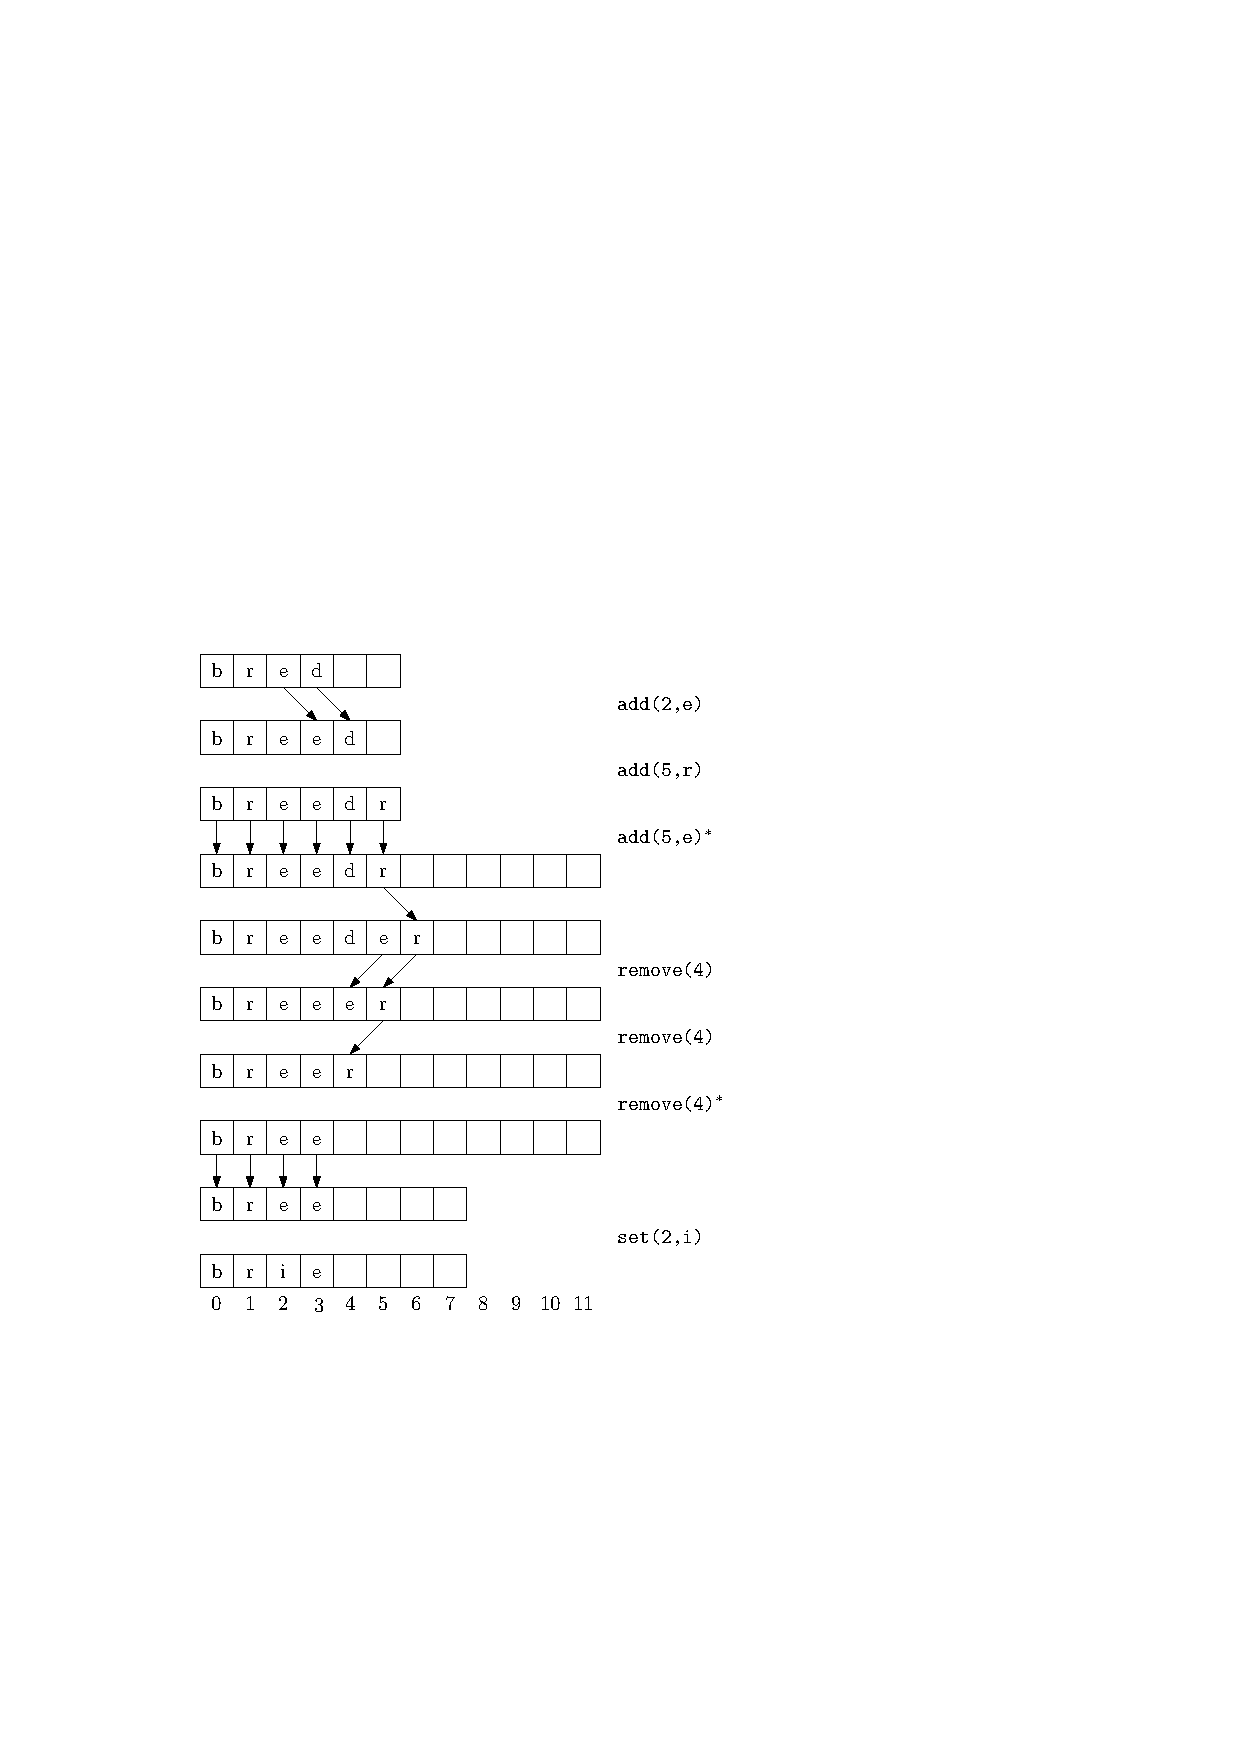
\includegraphics{figs/arraystack}
  \end{center}
  \caption{A sequence of \mbox{\texttt{add({\color{var}i},{\color{var}x})}} and \mbox{\texttt{remove({\color{var}i})}} operation in an
  \mbox{\texttt{ArrayStack}}.  Arrows denote elements being copied.  Operations that
  result in a call to \mbox{\texttt{resize()}} are marked with an asterisk.}
  \figlabel{arraystack}
\end{figure}

\begin{Verbatim}[tabsize=2,frame=single,commandchars=\\@\$,label=\texttt{ArrayStack},labelposition=topline]
	@\color@var$void$ add(@\color@keyword$int$ @\color@var$i$, @\color@keyword$T$ @\color@var$x$) {
		@\color@keyword$if$ (@\color@var$i$ < 0 || @\color@var$i$ > @\color@var$n$) @\color@keyword$throw$ @\color@keyword$new$ IndexOutOfBoundsException();
		@\color@keyword$if$ (@\color@var$n$ + 1 > @\color@var$a$.@\color@var$length$) resize();
		@\color@keyword$for$ (@\color@keyword$int$ @\color@var$j$ = @\color@var$n$; @\color@var$j$ > @\color@var$i$; @\color@var$j$--) 
			@\color@var$a$[@\color@var$j$] = @\color@var$a$[@\color@var$j$-1];
		@\color@var$a$[@\color@var$i$] = @\color@var$x$;
		@\color@var$n$++;
	}
\end{Verbatim}
% TODO: Add shifting figure
If we ignore the cost of the potential call to \mbox{\texttt{resize()}}, the cost of the
\mbox{\texttt{add({\color{var}i},{\color{var}x})}} operation is proportional to the number of elements we have
to shift to make room for \mbox{\texttt{{\color{var}x}}}.  Therefore the cost of this operation
(ignoring the cost of resizing \mbox{\texttt{{\color{var}a}}}) is $O(\mbox{\texttt{{\color{var}n}}}-\mbox{\texttt{{\color{var}i}}}+1)$.

Implementing the \mbox{\texttt{remove({\color{var}i})}} operation is similar.  We shift the elements
$\mbox{\texttt{{\color{var}a}[{\color{var}i}+1]}},\ldots,\mbox{\texttt{{\color{var}a}[{\color{var}n}-1]}}$ left by one position (overwriting \mbox{\texttt{{\color{var}a}[{\color{var}i}]}}) and
decrease the value of \mbox{\texttt{{\color{var}n}}}.  After doing this, we check if \mbox{\texttt{{\color{var}n}}} is getting
much smaller than \mbox{\texttt{{\color{var}a}.{\color{var}length}}} by checking if $\mbox{\texttt{{\color{var}a}.{\color{var}length}}} \ge 3\mbox{\texttt{{\color{var}n}}}$. If so,
we call \mbox{\texttt{resize()}} to reduce the size of \mbox{\texttt{{\color{var}a}}}.

\begin{Verbatim}[tabsize=2,frame=single,commandchars=\\@\$,label=\texttt{ArrayStack},labelposition=topline]
	@\color@keyword$T$ remove(@\color@keyword$int$ @\color@var$i$) {
		@\color@keyword$if$ (@\color@var$i$ < 0 || @\color@var$i$ > @\color@var$n$ - 1) @\color@keyword$throw$ @\color@keyword$new$ IndexOutOfBoundsException();
		@\color@keyword$T$ @\color@var$x$ = @\color@var$a$[@\color@var$i$];
		@\color@keyword$for$ (@\color@keyword$int$ @\color@var$j$ = @\color@var$i$; @\color@var$j$ < @\color@var$n$-1; @\color@var$j$++) 
			@\color@var$a$[@\color@var$j$] = @\color@var$a$[@\color@var$j$+1];
		@\color@var$n$--;
		@\color@keyword$if$ (@\color@var$a$.@\color@var$length$ >= 3*@\color@var$n$) resize();
		@\color@var$return$ @\color@var$x$;
	}
\end{Verbatim}
% TODO: Add shifting figure
If we ignore the cost of the \mbox{\texttt{resize()}} method, the cost of a \mbox{\texttt{remove({\color{var}i})}}
operation is proportional to the number of the number elements we shift,
which is $O(\mbox{\texttt{{\color{var}n}}}-\mbox{\texttt{{\color{var}i}}})$. 

\subsection{Growing and Shrinking}

The \mbox{\texttt{resize()}} method is fairly straightforward; it allocates a new
array \mbox{\texttt{{\color{var}b}}} whose size is $2\mbox{\texttt{{\color{var}n}}}$ and copies the \mbox{\texttt{{\color{var}n}}} elements of \mbox{\texttt{{\color{var}a}}} into
the first \mbox{\texttt{{\color{var}n}}} positions in \mbox{\texttt{{\color{var}b}}}, and then sets \mbox{\texttt{{\color{var}a}}} to \mbox{\texttt{{\color{var}b}}}. Thus, after a call to \mbox{\texttt{resize()}}, $\mbox{\texttt{{\color{var}a}.{\color{var}length}}} = 2\mbox{\texttt{{\color{var}n}}}$.

\begin{Verbatim}[tabsize=2,frame=single,commandchars=\\@\$,label=\texttt{ArrayStack},labelposition=topline]
	@\color@var$void$ resize() {
		@\color@keyword$T$[] @\color@var$b$ = newArray(max(@\color@var$n$*2,1));
		@\color@keyword$for$ (@\color@keyword$int$ @\color@var$i$ = 0; @\color@var$i$ < @\color@var$n$; @\color@var$i$++) {
			@\color@var$b$[@\color@var$i$] = @\color@var$a$[@\color@var$i$];
		}
		@\color@var$a$ = @\color@var$b$;
	}
\end{Verbatim}

Analyzing the actual cost of the \mbox{\texttt{resize()}} operation is easy. It
allocates an array \mbox{\texttt{{\color{var}b}}} of size $2\mbox{\texttt{{\color{var}n}}}$ and copies the \mbox{\texttt{{\color{var}n}}} elements of \mbox{\texttt{{\color{var}a}}}
into \mbox{\texttt{{\color{var}b}}}.  This takes $O(\mbox{\texttt{{\color{var}n}}})$ time.

The running time analysis from the previous section ignored the cost
of calls to \mbox{\texttt{resize()}}.  In this section we analyze this cost using a
technique known as \emph{amortized analysis}.  This technique does not
try and determine the cost of resizing during each individual \mbox{\texttt{add({\color{var}i},{\color{var}x})}}
and \mbox{\texttt{remove({\color{var}i})}} operation.  Instead, it considers the cost of all calls to
\mbox{\texttt{resize()}} during a sequence of $m$ calls to \mbox{\texttt{add({\color{var}i},{\color{var}x})}} or \mbox{\texttt{remove({\color{var}x})}}.
In particular, we will show:

\begin{lem}\lemlabel{arraystack-amortized}
  If an empty \mbox{\texttt{ArrayList}} is created and any sequence of $m\ge 1$ calls
  to \mbox{\texttt{add({\color{var}i},{\color{var}x})}} and \mbox{\texttt{remove({\color{var}i})}} are performed, then the total cost of all work
  done during all calls to \mbox{\texttt{resize()}} is $O(m)$.
\end{lem}

\begin{proof}
  We will show that anytime \mbox{\texttt{resize()}} is called, the number of calls
  to \mbox{\texttt{{\color{var}add}}} or \mbox{\texttt{{\color{var}remove}}} since the last call to \mbox{\texttt{resize()}} is at least
  $\mbox{\texttt{{\color{var}n}}}/2-1$.  Therefore, if $n_i$ denotes the value of \mbox{\texttt{{\color{var}n}}} during the $i$th
call to \mbox{\texttt{resize()}}, then the total number of calls to \mbox{\texttt{add({\color{var}i},{\color{var}x})}} or
\mbox{\texttt{remove({\color{var}i})}} is at least
  \[
     \sum_{i=1}^{r} (n_i/2-1) \le m  \enspace .
  \]
  On the other hand, the total work done during all calls to \mbox{\texttt{resize()}} is 
  \[
     \sum_{i=1}^{r} O(n_i) \le O(m+r) = O(m)  \enspace ,
  \]
  which will prove the theorem since $r$, the number of calls to
\mbox{\texttt{resize()}},
  is not more than $m$.  All that remains is to show that the number
  of calls to \mbox{\texttt{add({\color{var}i},{\color{var}x})}} or \mbox{\texttt{remove({\color{var}i})}} between the $(i-1)$th and the
  $i$th call to \mbox{\texttt{resize()}} is at least $n_i/2$.

  There are two cases to consider. In the first case, \mbox{\texttt{resize()}} is
  being called by \mbox{\texttt{add({\color{var}i},{\color{var}x})}} because the backing array \mbox{\texttt{{\color{var}a}}} is full, i.e.,
  $\mbox{\texttt{{\color{var}a}.length()}} = \mbox{\texttt{{\color{var}n}}}=n_i$.  Consider the previous call to \mbox{\texttt{resize()}}:
  After this previous call, the size of \mbox{\texttt{{\color{var}a}}} was \mbox{\texttt{{\color{var}a}.{\color{var}length}}}, but the
  number of elements stored in \mbox{\texttt{{\color{var}a}}} was at most $\mbox{\texttt{{\color{var}a}.{\color{var}length}}}/2=n_i/2$.
  But now the number of elements stored in \mbox{\texttt{{\color{var}a}}} is $n_i=\mbox{\texttt{{\color{var}a}.{\color{var}length}}}$,
  so there must have been at least $n_i/2$ calls to \mbox{\texttt{add({\color{var}i},{\color{var}x})}} since
  the previous call to \mbox{\texttt{resize()}}.
  % TODO: Add figure
  
  The second case to consider is when \mbox{\texttt{resize()}} is being called by
  \mbox{\texttt{remove({\color{var}i})}} because $\mbox{\texttt{{\color{var}a}.{\color{var}length}}} \ge 3\mbox{\texttt{{\color{var}n}}}=3n_i$.  Again, after the
  previous call to \mbox{\texttt{resize()}} the number of elements stored in \mbox{\texttt{{\color{var}a}}} was
  at least $\mbox{\texttt{{\color{var}a}.{\color{var}length}/2}}-1$. (The ${}-1$ in this formula accounts for
  the special case that occurs when $\mbox{\texttt{{\color{var}n}}}=0$ and \mbox{\texttt{{\color{var}a}.{\color{var}length}=1}}.) Now there
  are $n_i\le\mbox{\texttt{{\color{var}a}.{\color{var}length}}}/3$ elements stored in \mbox{\texttt{{\color{var}a}}}.  Therefore, the number
  of \mbox{\texttt{remove({\color{var}i})}} operations since the last call to \mbox{\texttt{resize()}} is at least
  \[
      \mbox{\texttt{{\color{var}a}.{\color{var}length}}}/2 - 1 - \mbox{\texttt{{\color{var}a}.{\color{var}length}}}/3 = \mbox{\texttt{{\color{var}a}.{\color{var}length}}}/6 - 1
         = (\mbox{\texttt{{\color{var}a}.{\color{var}length}}}/3)/2 - 1\ge n_i/2 -1\enspace .
  \]
  In either case, the number of calls to \mbox{\texttt{add({\color{var}i},{\color{var}x})}} or \mbox{\texttt{remove({\color{var}i})}} that
  occur between the $(i-1)$th call to \mbox{\texttt{resize()}} and the $i$th call to
  resize is at least $n_i/2-1$, as required to complete the proof.
\end{proof}

\subsection{Summary}

The following theorem summarizes the performance of an \mbox{\texttt{ArrayStack}}:

\begin{thm}\thmlabel{arraystack}
  An \mbox{\texttt{ArrayStack}} implements the \mbox{\texttt{List}} interface.  Ignoring the cost of
  calls to \mbox{\texttt{resize()}}, an \mbox{\texttt{ArrayStack}} supports the operations
  \begin{itemize}
    \item \mbox{\texttt{get({\color{var}i})}} and \mbox{\texttt{set({\color{var}i},{\color{var}x})}} in $O(1)$ time per operation; and
    \item \mbox{\texttt{add({\color{var}i},{\color{var}x})}} and \mbox{\texttt{remove({\color{var}i})}} in $O(1+\mbox{\texttt{{\color{var}n}}}-\mbox{\texttt{{\color{var}i}}})$ time per operation.
  \end{itemize}
  Furthermore, beginning with an empty \mbox{\texttt{ArrayStack}}, any sequence of $m$
  \mbox{\texttt{add({\color{var}i},{\color{var}x})}} and \mbox{\texttt{remove({\color{var}i})}} operations results in a total of $O(m)$
  work during all calls to \mbox{\texttt{resize()}}.
\end{thm}

The \mbox{\texttt{ArrayStack}} is an efficient way to implement a \mbox{\texttt{Stack}}.
In particular, we can implement \mbox{\texttt{push({\color{var}x})}} as \mbox{\texttt{add({\color{var}n},{\color{var}x})}} and \mbox{\texttt{pop()}}
as \mbox{\texttt{remove({\color{var}n}-1)}}, in which case these operations will run in $O(1)$
amortized time.

\section{\mbox{\texttt{FastArrayStack}}: An Optimized ArrayStack}
\seclabel{fastarraystack}
Much of the work done by an \mbox{\texttt{ArrayStack}} involves shifting (by
\mbox{\texttt{add({\color{var}i},{\color{var}x})}} and \mbox{\texttt{remove({\color{var}i})}}) and copying (by \mbox{\texttt{resize()}}) of data.  In the
implementations shown above, this was done using \mbox{\texttt{{\color{keyword}for}}} loops. It turns
out that many programming environments have specific functions that are
very efficient at copying and moving blocks of data.  In the C and C++
programming languages there is the \mbox{\texttt{memcpy({\color{var}d},{\color{var}s},{\color{var}n})}} function.  In Java
there is the \mbox{\texttt{System.arraycopy({\color{var}s},{\color{var}i},{\color{var}d},{\color{var}j},{\color{var}n})}} method.

\begin{Verbatim}[tabsize=2,frame=single,commandchars=\\@\$,label=\texttt{FastArrayStack},labelposition=topline]
	@\color@var$void$ resize() {
		@\color@keyword$T$[] @\color@var$b$ = newArray(max(2*@\color@var$n$,1));
		System.arraycopy(@\color@var$a$, 0, @\color@var$b$, 0, @\color@var$n$);
		@\color@var$a$ = @\color@var$b$;
	}
	@\color@var$void$ add(@\color@keyword$int$ @\color@var$i$, @\color@keyword$T$ @\color@var$x$) {
		@\color@keyword$if$ (@\color@var$i$ < 0 || @\color@var$i$ > @\color@var$n$) @\color@keyword$throw$ @\color@keyword$new$ IndexOutOfBoundsException();
		@\color@keyword$if$ (@\color@var$n$ + 1 > @\color@var$a$.@\color@var$length$) resize();
		System.arraycopy(@\color@var$a$, @\color@var$i$, @\color@var$a$, @\color@var$i$+1, @\color@var$n$-@\color@var$i$); 
		@\color@var$a$[@\color@var$i$] = @\color@var$x$;
		@\color@var$n$++;
	}
	@\color@keyword$T$ remove(@\color@keyword$int$ @\color@var$i$) {
		@\color@keyword$if$ (@\color@var$i$ < 0 || @\color@var$i$ > @\color@var$n$ - 1) @\color@keyword$throw$ @\color@keyword$new$ IndexOutOfBoundsException();
		@\color@keyword$T$ @\color@var$x$ = @\color@var$a$[@\color@var$i$];
		System.arraycopy(@\color@var$a$, @\color@var$i$+1, @\color@var$a$, @\color@var$i$, @\color@var$n$-@\color@var$i$-1);
		@\color@var$n$--; 
		@\color@keyword$if$ (@\color@var$a$.@\color@var$length$ >= 3*@\color@var$n$) resize();
		@\color@var$return$ @\color@var$x$;
	}
\end{Verbatim}

These functions are usually highly optimized and may even use special
machine instructions that can do this copying much faster than we could do
with \mbox{\texttt{{\color{keyword}for}}} loop.  Although using these functions does not asymptotically
decrease the running times, it can still be a worthwhile optimization.
In the Java implementations here, the use of \mbox{\texttt{System.arraycopy({\color{var}s},{\color{var}i},{\color{var}d},{\color{var}j},{\color{var}n})}}
resulted in speedups of a factor of 2-3 depending on the types of
operations performed.

\section{\mbox{\texttt{ArrayQueue}}: An Array-Based Queue}
\seclabel{arrayqueue}

In this section, we present the \mbox{\texttt{ArrayQueue}} data structure, which
implements a FIFO (first-in-first-out) queue; elements are removed (using
the \mbox{\texttt{remove()}} operation) from the queue in the same order they are added
(using the \mbox{\texttt{add({\color{var}x})}} operation).

Notice that an \mbox{\texttt{ArrayStack}} is a poor choice for an implementation of a
FIFO queue.  The reason is that we must choose one end of the list to
add to and then remove from the other end.  One of the two operations
must work on the head of the list, which involves calling \mbox{\texttt{add({\color{var}i},{\color{var}x})}}
or \mbox{\texttt{remove({\color{var}i})}} with a value of $\mbox{\texttt{{\color{var}i}}}=0$.  This gives a running time
of $\Theta(n)$.

To obtain an efficient array-based implementation of a queue, we
first notice that the problem would be easy if we had an infinite
array \mbox{\texttt{{\color{var}a}}}.  We could maintain one index \mbox{\texttt{{\color{var}j}}} that keeps track of the
next element to remove and an integer \mbox{\texttt{{\color{var}n}}} that counts the number of
elements in the queue.  The queue elements would always be stored in
\[ \mbox{\texttt{{\color{var}a}[{\color{var}j}]}},\mbox{\texttt{{\color{var}a}[{\color{var}j}+1]}},\ldots,\mbox{\texttt{{\color{var}a}[{\color{var}j}+{\color{var}n}-1]}} \enspace . \]
Initially, both \mbox{\texttt{{\color{var}i}}} and \mbox{\texttt{{\color{var}n}}} would be 
set to 0.  To add an element, we would place it in \mbox{\texttt{{\color{var}a}[{\color{var}j}+{\color{var}n}]}} and increment \mbox{\texttt{{\color{var}n}}}.
To remove an element, we would remove it from \mbox{\texttt{{\color{var}a}[{\color{var}j}]}}, increment \mbox{\texttt{{\color{var}j}}}, and
decrement \mbox{\texttt{{\color{var}n}}}.

Of course, the problem with this solution is that it requires an infinite
array \mbox{\texttt{{\color{var}a}}}.  An \mbox{\texttt{ArrayQueue}} simulates this by using a finite array \mbox{\texttt{{\color{var}a}}}
and \emph{modular arithmetic}.  This is the kind of arithmetic used when
we are talking about time of day.  For example 10 o'clock plus 5
hours gives 3 o'clock.  Formally, we say that
\[
    10 + 5 = 15 \equiv 3 \pmod{12} \enspace .
\]
We read the latter part of this equation as ``15 is congruent to 3 modulo
12.'' We can also treat $\bmod$ as binary operator, so that
\[
   15 \bmod 12 = 3 \enspace .
\]

More generally, for an integer $a$ and positive integer $m$, $a \bmod m$
is the unique integer $r\in\{0,\ldots,m-1\}$ such that $a = r + km$ for
some integer $k$.  Less formally, the value $r$ is the remainder we get
when we divide $a$ by $m$.  In many programming languages, including Java,
the $\bmod$ operator is represented using the \mbox{\texttt{\%}} symbol.\footnote{This
is sometimes referred to as the \emph{brain-dead} mod operator since
it does not correctly implement the mathematical mod operator when the
first argument is negative.}

Modular arithmetic is useful for simulating an infinite array,
since $\mbox{\texttt{{\color{var}i}}}\bmod \mbox{\texttt{{\color{var}a}.{\color{var}length}}}$ always gives a value in the range
$0,\ldots,\mbox{\texttt{{\color{var}a}.{\color{var}length}-1}}$.  Using modular arithmetic we can store the
queue elements at array locations
\[ \mbox{\texttt{{\color{var}a}[{\color{var}j}\%{\color{var}a}.{\color{var}length}]}},\mbox{\texttt{{\color{var}a}[({\color{var}j}+1)\%{\color{var}a}.{\color{var}length}]}},\ldots,\mbox{\texttt{{\color{var}a}[({\color{var}j}+{\color{var}n}-1)\%{\color{var}a}.{\color{var}length}]}}
\enspace. \]
This treats \mbox{\texttt{{\color{var}a}}} like a \emph{circular array} in which array indices
exceeding $\mbox{\texttt{{\color{var}a}.{\color{var}length}}}-1$ ``wrap around'' to the beginning of
the array.
% TODO: figure

The only remaining thing to worry about is taking care that the number
of elements in the \mbox{\texttt{ArrayQueue}} does not exceed the size of \mbox{\texttt{{\color{var}a}}}.

\begin{Verbatim}[tabsize=2,frame=single,commandchars=\\@\$,label=\texttt{ArrayQueue},labelposition=topline]
	@\color@keyword$T$[] @\color@var$a$;
	@\color@keyword$int$ @\color@var$j$;
	@\color@keyword$int$ @\color@var$n$;
\end{Verbatim}

A sequence of \mbox{\texttt{add({\color{var}x})}} and \mbox{\texttt{remove()}} operation on an \mbox{\texttt{ArrayQueue}} are illusted in \figref{arrayqueue}.
To implement \mbox{\texttt{add({\color{var}x})}}, we first check if \mbox{\texttt{{\color{var}a}}} is full and, if necessary,
call \mbox{\texttt{resize()}} to increase the size of \mbox{\texttt{{\color{var}a}}}.  Next, we store \mbox{\texttt{{\color{var}x}}} in
\mbox{\texttt{{\color{var}a}[({\color{var}j}+{\color{var}n})\%{\color{var}a}.{\color{var}length}]}} and increment \mbox{\texttt{{\color{var}n}}}.

\begin{figure}
  \begin{center}
    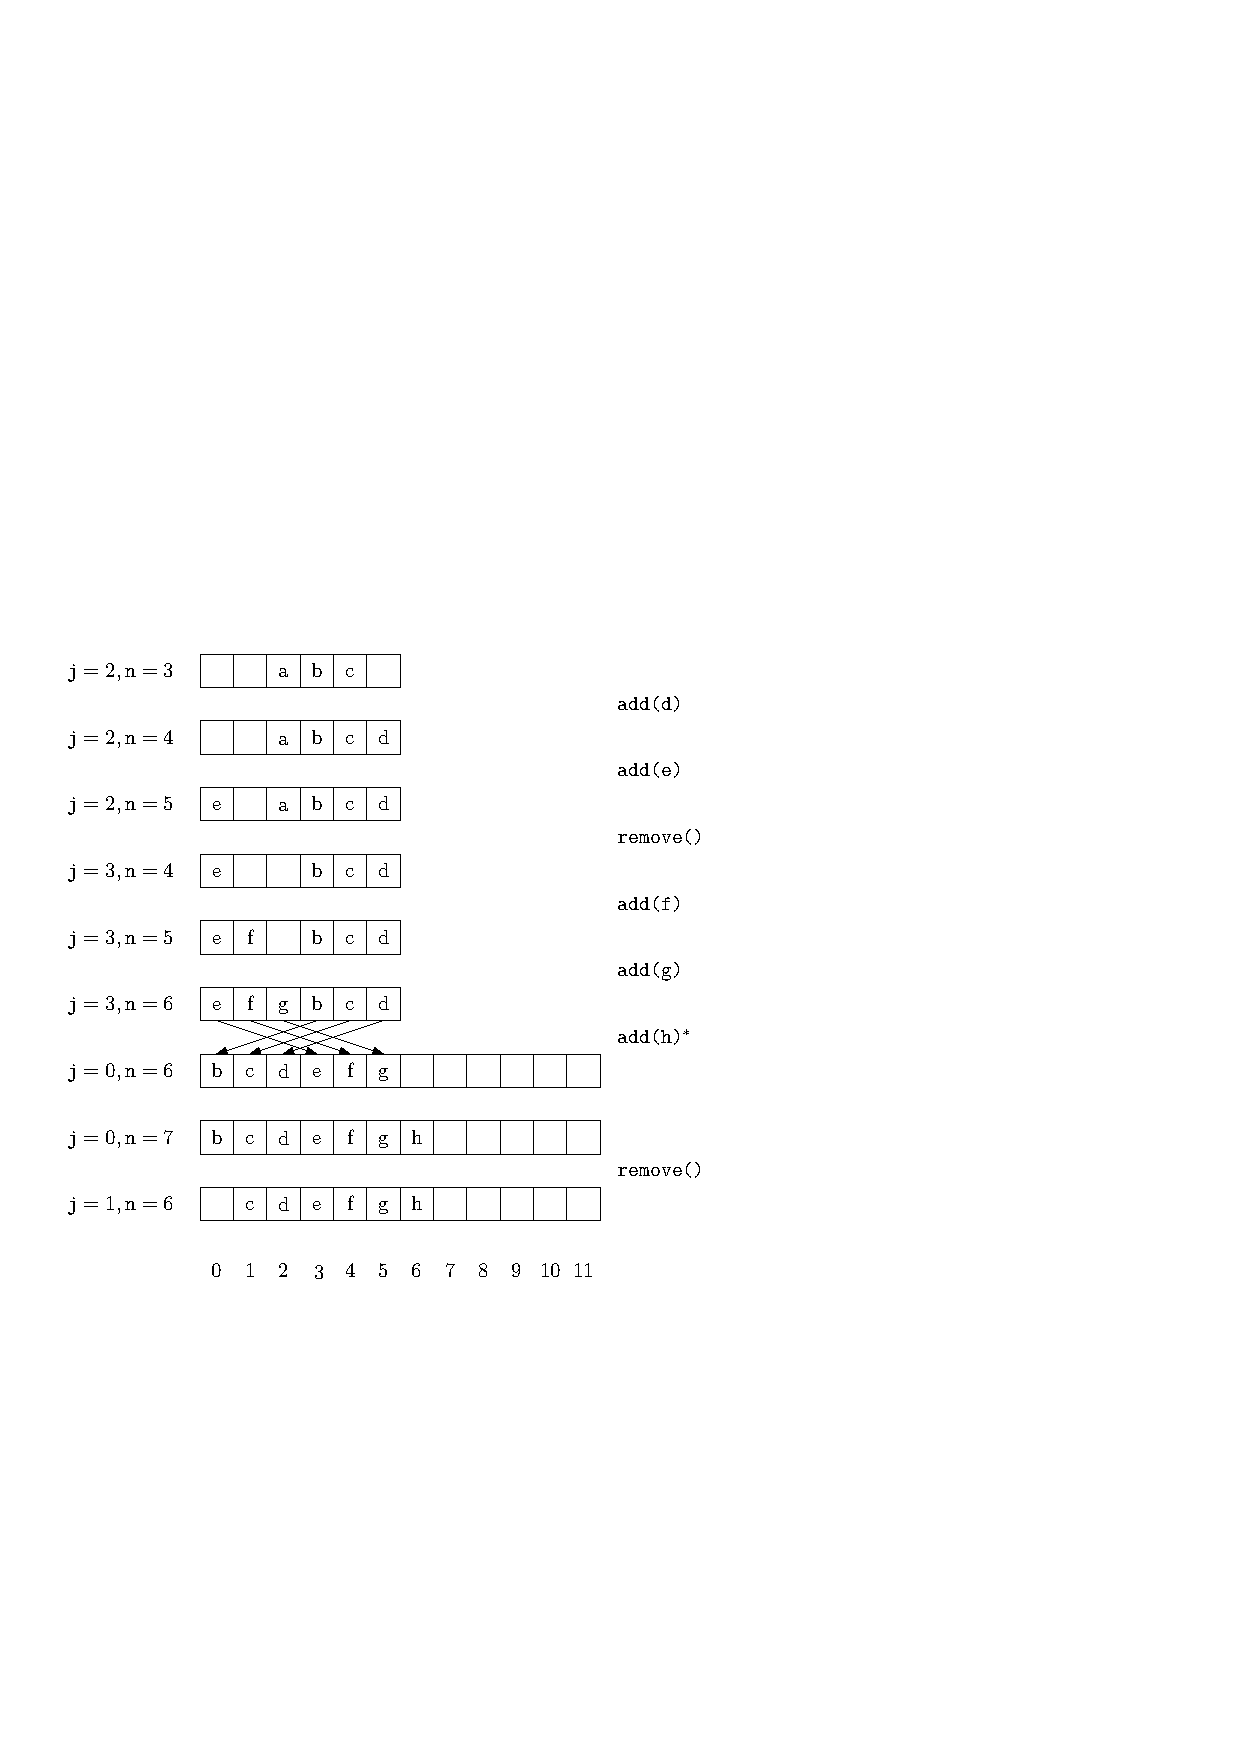
\includegraphics{figs/arrayqueue}
  \end{center}
  \caption{A sequence of \mbox{\texttt{add({\color{var}x})}} and \mbox{\texttt{remove({\color{var}i})}} operation on an
  \mbox{\texttt{ArrayQueue}}.  Arrows denote elements being copied.  Operations that
  result in a call to \mbox{\texttt{resize()}} are marked with an asterisk.}
  \figlabel{arrayqueue}
\end{figure}



\begin{Verbatim}[tabsize=2,frame=single,commandchars=\\@\$,label=\texttt{ArrayQueue},labelposition=topline]
	@\color@var$boolean$ add(@\color@keyword$T$ @\color@var$x$) {
		@\color@keyword$if$ (@\color@var$n$ + 1 > @\color@var$a$.@\color@var$length$) resize();
		@\color@var$a$[(@\color@var$j$+@\color@var$n$) % @\color@var$a$.@\color@var$length$] = @\color@var$x$;
		@\color@var$n$++;
		@\color@var$return$ @\color@var$true$;
	}
\end{Verbatim}

To implement \mbox{\texttt{remove()}} we first store \mbox{\texttt{{\color{var}a}[{\color{var}j}]}} so that we can return
it later.  Next, we decrement \mbox{\texttt{{\color{var}n}}} and ``increment'' \mbox{\texttt{{\color{var}j}}} by setting
$\mbox{\texttt{{\color{var}j}}}=(\mbox{\texttt{{\color{var}j}}}+1)\bmod \mbox{\texttt{{\color{var}a}.{\color{var}length}}}$ and return the stored value of \mbox{\texttt{{\color{var}a}[{\color{var}j}]}}. If
necessary, we may call \mbox{\texttt{resize()}} to decrease the size of \mbox{\texttt{{\color{var}a}}}.

\begin{Verbatim}[tabsize=2,frame=single,commandchars=\\@\$,label=\texttt{ArrayQueue},labelposition=topline]
	@\color@keyword$T$ remove() { 
		@\color@keyword$if$ (@\color@var$n$ == 0) @\color@keyword$throw$ @\color@keyword$new$ NoSuchElementException();
		@\color@keyword$T$ @\color@var$x$ = @\color@var$a$[@\color@var$j$];
		@\color@var$j$ = (@\color@var$j$ + 1) % @\color@var$a$.@\color@var$length$;
		@\color@var$n$--;
		@\color@keyword$if$ (@\color@var$a$.@\color@var$length$ >= 3*@\color@var$n$) resize();
		@\color@var$return$ @\color@var$x$;
	}
\end{Verbatim}

Finally, the \mbox{\texttt{resize()}} operation is very similar to the \mbox{\texttt{resize()}}
operation of \mbox{\texttt{ArrayQueue}}.  It allocates a new array \mbox{\texttt{{\color{var}b}}} of size $2\mbox{\texttt{{\color{var}n}}}$
and copies
\[
   \mbox{\texttt{{\color{var}a}[{\color{var}j}]}},\mbox{\texttt{{\color{var}a}[({\color{var}j}+1)\%{\color{var}a}.{\color{var}length}]}},\ldots,\mbox{\texttt{{\color{var}a}[({\color{var}j}+{\color{var}n}-1)\%{\color{var}a}.{\color{var}length}]}}
\]
onto
\[
   \mbox{\texttt{{\color{var}b}[0]}},\mbox{\texttt{{\color{var}b}[1]}},\ldots,\mbox{\texttt{{\color{var}b}[{\color{var}n}-1]}}
\]
and sets $\mbox{\texttt{{\color{var}j}}}=0$.

\begin{Verbatim}[tabsize=2,frame=single,commandchars=\\@\$,label=\texttt{ArrayQueue},labelposition=topline]
	@\color@var$void$ resize() {
		@\color@keyword$T$[] @\color@var$b$ = newArray(max(1,@\color@var$n$*2));
		@\color@keyword$for$ (@\color@keyword$int$ @\color@var$k$ = 0; @\color@var$k$ < @\color@var$n$; @\color@var$k$++) 
			@\color@var$b$[@\color@var$k$] = @\color@var$a$[(@\color@var$j$+@\color@var$k$) % @\color@var$a$.@\color@var$length$];
		@\color@var$a$ = @\color@var$b$;
		@\color@var$j$ = 0;
	}
\end{Verbatim}

\subsection{Summary}

The following theorem summarizes the performance of the \mbox{\texttt{ArrayQueue}}
data structure:

\begin{thm}
An \mbox{\texttt{ArrayQueue}} implements the (FIFO) \mbox{\texttt{Queue}} interface.  Ignoring the cost of
calls to \mbox{\texttt{resize()}}, an \mbox{\texttt{ArrayQueue}} supports the operations
\mbox{\texttt{add({\color{var}x})}} and \mbox{\texttt{remove()}} in $O(1)$ time per operation.
Furthermore, beginning with an empty \mbox{\texttt{ArrayQueue}}, any sequence of $m$
\mbox{\texttt{add({\color{var}i},{\color{var}x})}} and \mbox{\texttt{remove({\color{var}i})}} operations results in a total of $O(m)$
work during all calls to \mbox{\texttt{resize()}}.
\end{thm}

%TODO: Discuss the use of bitwise-and as a replacement for the mod operator

\section{\mbox{\texttt{ArrayDeque}}: Fast Deque Operations Using an Array}
\seclabel{arraydeque}

The \mbox{\texttt{ArrayQueue}} from the previous section gives data structure for
representing a sequence that allows us to efficiently add to one end
of the sequence and remove from the other end.  The \mbox{\texttt{ArrayDeque}} data
structure uses the same technique, but allows for efficient addition or
removal at both ends.  This structure implements the \mbox{\texttt{List}} interface
using the same circular array technique used to represent an \mbox{\texttt{ArrayQueue}}.

\begin{Verbatim}[tabsize=2,frame=single,commandchars=\\@\$,label=\texttt{ArrayDeque},labelposition=topline]
	@\color@keyword$T$[] @\color@var$a$;
	@\color@keyword$int$ @\color@var$j$;
	@\color@keyword$int$ @\color@var$n$;
\end{Verbatim}

The \mbox{\texttt{get({\color{var}i})}} and \mbox{\texttt{set({\color{var}i},{\color{var}x})}} operations in an \mbox{\texttt{ArrayDeque}} are
straightforward.  They get or set the array element $\mbox{\texttt{{\color{var}a}[}}{\mbox{\texttt{({\color{var}j}+{\color{var}i})}}\bmod
\mbox{\texttt{{\color{var}a}.{\color{var}length}}}}\mbox{\texttt{]}}$.

\begin{Verbatim}[tabsize=2,frame=single,commandchars=\\@\$,label=\texttt{ArrayDeque},labelposition=topline]
	@\color@keyword$T$ get(@\color@keyword$int$ @\color@var$i$) {
		@\color@keyword$if$ (@\color@var$i$ < 0 || @\color@var$i$ > @\color@var$n$-1) @\color@keyword$throw$ @\color@keyword$new$ IndexOutOfBoundsException();
		@\color@var$return$ @\color@var$a$[(@\color@var$j$+@\color@var$i$)%@\color@var$a$.@\color@var$length$];
	}
	@\color@keyword$T$ set(@\color@keyword$int$ @\color@var$i$, @\color@keyword$T$ @\color@var$x$) {
		@\color@keyword$if$ (@\color@var$i$ < 0 || @\color@var$i$ > @\color@var$n$-1) @\color@keyword$throw$ @\color@keyword$new$ IndexOutOfBoundsException();
		@\color@keyword$T$ @\color@var$y$ = @\color@var$a$[(@\color@var$j$+@\color@var$i$)%@\color@var$a$.@\color@var$length$];
		@\color@var$a$[(@\color@var$j$+@\color@var$i$)%@\color@var$a$.@\color@var$length$] = @\color@var$x$;
		@\color@var$return$ @\color@var$y$;
	}
\end{Verbatim}

Adding and removing elements from an \mbox{\texttt{ArrayDeque}} is illustrated in
\figref{arraydeque}.  The implementation of \mbox{\texttt{add({\color{var}i},{\color{var}x})}} is a little
more interesting.   As usual, we first check if \mbox{\texttt{{\color{var}a}}} is full and,
if necessary, call \mbox{\texttt{resize()}} to resize \mbox{\texttt{{\color{var}a}}}.   Remember that we want
this operation to be fast when \mbox{\texttt{{\color{var}i}}} is small (close to 0) or when \mbox{\texttt{{\color{var}i}}}
is large (close to \mbox{\texttt{{\color{var}n}}}).  Therefore, we check if $\mbox{\texttt{{\color{var}i}}}<\mbox{\texttt{{\color{var}n}}}/2$.  If so,
we shift the elements $\mbox{\texttt{{\color{var}a}[0]}},\ldots,\mbox{\texttt{{\color{var}a}[{\color{var}i}-1]}}$ left by one position.
Otherwise ($\mbox{\texttt{{\color{var}i}}}\ge\mbox{\texttt{{\color{var}n}}}/2$), we shift the elements $\mbox{\texttt{{\color{var}a}[{\color{var}i}]}},\ldots,\mbox{\texttt{{\color{var}a}[{\color{var}n}-1]}}$
right by one position.

\begin{figure}
  \begin{center}
    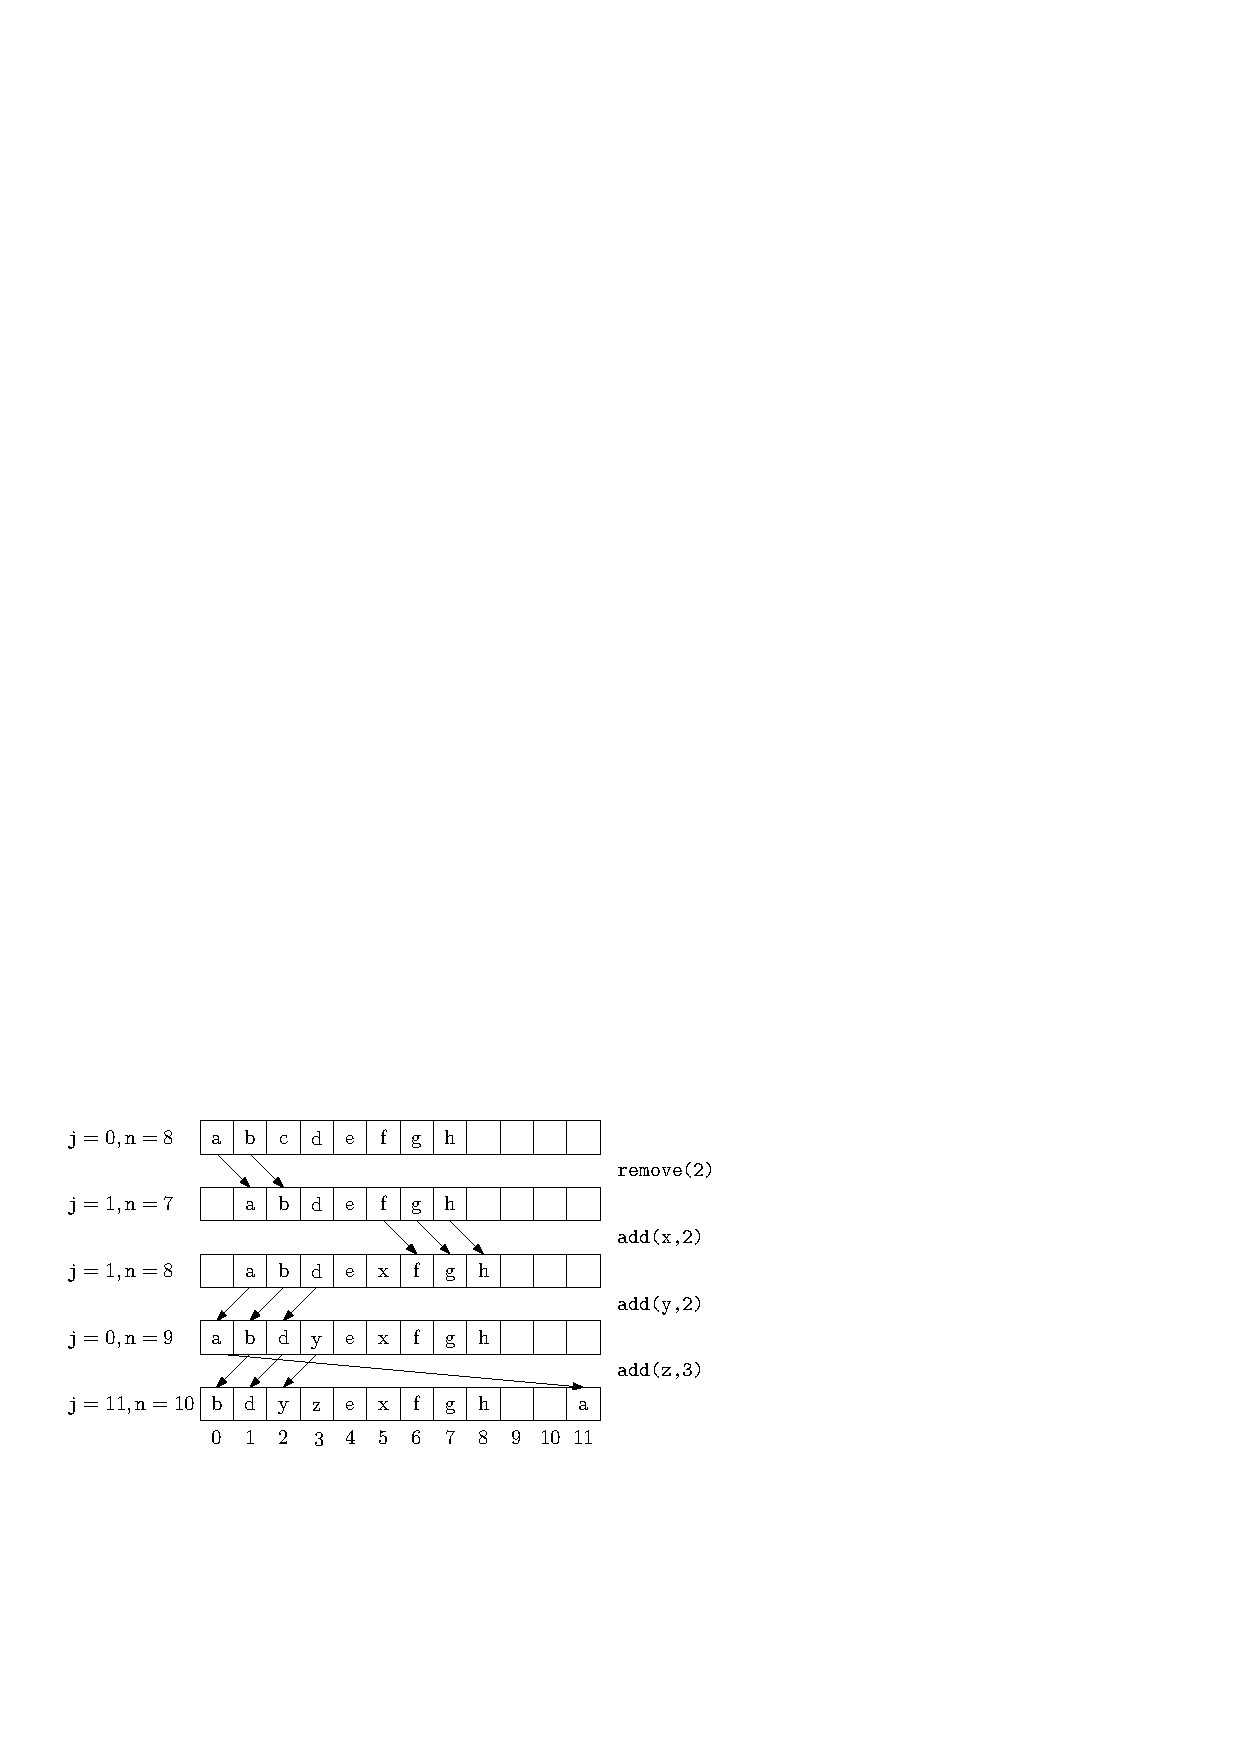
\includegraphics{figs/arraydeque}
  \end{center}
  \caption{A sequence of \mbox{\texttt{add({\color{var}i},{\color{var}x})}} and \mbox{\texttt{remove({\color{var}i})}} operation in an
  \mbox{\texttt{ArrayDeque}}.  Arrows denote elements being copied.}
  \figlabel{arraydeque}
\end{figure}


\begin{Verbatim}[tabsize=2,frame=single,commandchars=\\@\$,label=\texttt{ArrayDeque},labelposition=topline]
	@\color@var$void$ add(@\color@keyword$int$ @\color@var$i$, @\color@keyword$T$ @\color@var$x$) {
		@\color@keyword$if$ (@\color@var$i$ < 0 || @\color@var$i$ > @\color@var$n$) @\color@keyword$throw$ @\color@keyword$new$ IndexOutOfBoundsException();
		@\color@keyword$if$ (@\color@var$n$+1 > @\color@var$a$.@\color@var$length$) resize();
		@\color@keyword$if$ (@\color@var$i$ < @\color@var$n$/2) {	@\color@comment$// shift a[0],..,a[i-1] left one position$
			@\color@var$j$ = (@\color@var$j$ == 0) ? @\color@var$a$.@\color@var$length$ - 1 : @\color@var$j$ - 1;
			@\color@keyword$for$ (@\color@keyword$int$ @\color@var$k$ = 0; @\color@var$k$ <= @\color@var$i$-1; @\color@var$k$++)
				@\color@var$a$[(@\color@var$j$+@\color@var$k$)%@\color@var$a$.@\color@var$length$] = @\color@var$a$[(@\color@var$j$+@\color@var$k$+1)%@\color@var$a$.@\color@var$length$];
		} @\color@keyword$else$ {	    @\color@comment$// shift a[i],..,a[n-1] right one position$
			@\color@keyword$for$ (@\color@keyword$int$ @\color@var$k$ = @\color@var$n$; @\color@var$k$ > @\color@var$i$; @\color@var$k$--)
				@\color@var$a$[(@\color@var$j$+@\color@var$k$)%@\color@var$a$.@\color@var$length$] = @\color@var$a$[(@\color@var$j$+@\color@var$k$-1)%@\color@var$a$.@\color@var$length$];
		}
		@\color@var$a$[(@\color@var$j$+@\color@var$i$)%@\color@var$a$.@\color@var$length$] = @\color@var$x$;
		@\color@var$n$++;
	}
\end{Verbatim}

By doing the shifting in this way, we guarantee that \mbox{\texttt{add({\color{var}i},{\color{var}x})}} never
has to shift more than $\min\{ \mbox{\texttt{{\color{var}i}}}, \mbox{\texttt{{\color{var}n}}}-\mbox{\texttt{{\color{var}i}}} \}$ elements.  Thus, the running
time of the \mbox{\texttt{add({\color{var}i},{\color{var}x})}} operation (ignoring the cost of the \mbox{\texttt{resize()}}
operation) is $O(1+\min\{\mbox{\texttt{{\color{var}i}}},\mbox{\texttt{{\color{var}n}}}-\mbox{\texttt{{\color{var}i}}}\})$.

The \mbox{\texttt{remove({\color{var}i})}} operation is similar.  It either shifts elements
$\mbox{\texttt{{\color{var}a}[0]}},\ldots,\mbox{\texttt{{\color{var}a}[{\color{var}i}-1]}}$ right by one position or shifts the elements
$\mbox{\texttt{{\color{var}a}[{\color{var}i}+1]}},\ldots,\mbox{\texttt{{\color{var}a}[{\color{var}n}-1]}}$ left by one position depending on whether
$\mbox{\texttt{{\color{var}i}}}<\mbox{\texttt{{\color{var}n}}}/2$.  Again, this means that \mbox{\texttt{remove({\color{var}i})}} never does more than 
$O(1+\min\{\mbox{\texttt{{\color{var}i}}},\mbox{\texttt{{\color{var}n}}}-\mbox{\texttt{{\color{var}i}}}\})$ work to shift elements.

\begin{Verbatim}[tabsize=2,frame=single,commandchars=\\@\$,label=\texttt{ArrayDeque},labelposition=topline]
	@\color@keyword$T$ remove(@\color@keyword$int$ @\color@var$i$) {
		@\color@keyword$if$ (@\color@var$i$ < 0 || @\color@var$i$ > @\color@var$n$ - 1)	@\color@keyword$throw$ @\color@keyword$new$ IndexOutOfBoundsException();
		@\color@keyword$T$ @\color@var$x$ = @\color@var$a$[(@\color@var$j$+@\color@var$i$)%@\color@var$a$.@\color@var$length$];
		@\color@keyword$if$ (@\color@var$i$ < @\color@var$n$/2) {  @\color@comment$// shift a[0],..,[i-1] right one position$
			@\color@keyword$for$ (@\color@keyword$int$ @\color@var$k$ = @\color@var$i$; @\color@var$k$ > 0; @\color@var$k$--)
				@\color@var$a$[(@\color@var$j$+@\color@var$k$)%@\color@var$a$.@\color@var$length$] = @\color@var$a$[(@\color@var$j$+@\color@var$k$-1)%@\color@var$a$.@\color@var$length$];
			@\color@var$j$ = (@\color@var$j$ + 1) % @\color@var$a$.@\color@var$length$;
		} @\color@keyword$else$ {        @\color@comment$// shift a[i+1],..,a[n-1] left one position$
			@\color@keyword$for$ (@\color@keyword$int$ @\color@var$k$ = @\color@var$i$; @\color@var$k$ < @\color@var$n$-1; @\color@var$k$++)
				@\color@var$a$[(@\color@var$j$+@\color@var$k$)%@\color@var$a$.@\color@var$length$] = @\color@var$a$[(@\color@var$j$+@\color@var$k$+1)%@\color@var$a$.@\color@var$length$];
		}
		@\color@var$n$--;
		@\color@keyword$if$ (3*@\color@var$n$ < @\color@var$a$.@\color@var$length$) resize();
		@\color@var$return$ @\color@var$x$;
	}
\end{Verbatim}

\subsection{Summary}

The following theorem summarizes the performance of the \mbox{\texttt{ArrayDeque}}
data structure:
\begin{thm}\thmlabel{arraydeque}
  An \mbox{\texttt{ArrayDeque}} implements the \mbox{\texttt{List}} interface.  Ignoring the cost of
  calls to \mbox{\texttt{resize()}}, an \mbox{\texttt{ArrayDeque}} supports the operations
  \begin{itemize}
    \item \mbox{\texttt{get({\color{var}i})}} and \mbox{\texttt{set({\color{var}i},{\color{var}x})}} in $O(1)$ time per operation; and
    \item \mbox{\texttt{add({\color{var}i},{\color{var}x})}} and \mbox{\texttt{remove({\color{var}i})}} in $O(1+\min\{\mbox{\texttt{{\color{var}i}}},\mbox{\texttt{{\color{var}n}}}-\mbox{\texttt{{\color{var}i}}}\})$ time
          per operation.
  \end{itemize}
  Furthermore, beginning with an empty \mbox{\texttt{ArrayDeque}}, any sequence of $m$
  \mbox{\texttt{add({\color{var}i},{\color{var}x})}} and \mbox{\texttt{remove({\color{var}i})}} operations results in a total of $O(m)$
  work during all calls to \mbox{\texttt{resize()}}.
\end{thm}

\section{\mbox{\texttt{DualArrayDeque}}: Buiding a Deque from Two Stacks}
\seclabel{dualarraydeque}

Next, we present another data structure, the \mbox{\texttt{DualArrayDeque}} that
achieves the same performance bounds as an \mbox{\texttt{ArrayDeque}} by using
two \mbox{\texttt{ArrayStack}}s.  Although the asymptotic performance of the
\mbox{\texttt{DualArrayDeque}} is no better than that of the \mbox{\texttt{ArrayDeque}}, it is
still worth studying since it offer a good example of how to make a
sophisticated data structure by combining two simpler data structures.

A \mbox{\texttt{DualArrayDeque}} represents a list using two \mbox{\texttt{ArrayStack}}s.  Recall that
an \mbox{\texttt{ArrayStack}} is fast when the operations on it modify elements near
the end.  A \mbox{\texttt{DualArrayDeque}} places two \mbox{\texttt{ArrayStack}}s, called \mbox{\texttt{{\color{var}front}}}
and \mbox{\texttt{{\color{var}back}}}, back-to-back so that operations are fast at either end.

\begin{Verbatim}[tabsize=2,frame=single,commandchars=\\@\$,label=\texttt{DualArrayDeque},labelposition=topline]
	List<@\color@keyword$T$> @\color@var$front$;
	List<@\color@keyword$T$> @\color@var$back$;
\end{Verbatim}

A \mbox{\texttt{DualArrayDeque}} does not explicitly store the number, \mbox{\texttt{{\color{var}n}}},
of elements it contains.  It doesn't need to, since it contains
$\mbox{\texttt{{\color{var}n}}}=\mbox{\texttt{{\color{var}front}.size()}} + \mbox{\texttt{{\color{var}back}.size()}}$ elements.  Nevertheless, when
analyzing the \mbox{\texttt{DualArrayDeque}} we will still use \mbox{\texttt{{\color{var}n}}} to denote the number
of elements it contains.

\begin{Verbatim}[tabsize=2,frame=single,commandchars=\\@\$,label=\texttt{DualArrayDeque},labelposition=topline]
	@\color@keyword$int$ size() {
		@\color@var$return$ @\color@var$front$.size() + @\color@var$back$.size();		
	}
\end{Verbatim}

The \mbox{\texttt{{\color{var}front}}} \mbox{\texttt{ArrayStack}} contains list elements with indices
$0,\ldots,\mbox{\texttt{{\color{var}front}.size()}}-1$, but stores them in reverse order.
The \mbox{\texttt{{\color{var}back}}} \mbox{\texttt{ArrayStack}} contains list elements with indices
$\mbox{\texttt{{\color{var}front}.size()}},\ldots,\mbox{\texttt{size()}}-1$ in the normal order.  In this way,
\mbox{\texttt{get({\color{var}i})}} and \mbox{\texttt{set({\color{var}i},{\color{var}x})}} translate into appropriate calls to \mbox{\texttt{get({\color{var}i})}}
or \mbox{\texttt{set({\color{var}i},{\color{var}x})}} on either \mbox{\texttt{{\color{var}front}}} or \mbox{\texttt{{\color{var}back}}}, which take $O(1)$ time per operation.

\begin{Verbatim}[tabsize=2,frame=single,commandchars=\\@\$,label=\texttt{DualArrayDeque},labelposition=topline]
	@\color@keyword$T$ get(@\color@keyword$int$ @\color@var$i$) {
		@\color@keyword$if$ (@\color@var$i$ < @\color@var$front$.size()) {
			@\color@var$return$ @\color@var$front$.get(@\color@var$front$.size()-@\color@var$i$-1);
		} @\color@keyword$else$ {
			@\color@var$return$ @\color@var$back$.get(@\color@var$i$-@\color@var$front$.size());
		}
	}
	@\color@keyword$T$ set(@\color@keyword$int$ @\color@var$i$, @\color@keyword$T$ @\color@var$x$) {
		@\color@keyword$if$ (@\color@var$i$ < @\color@var$front$.size()) {
			@\color@var$return$ @\color@var$front$.set(@\color@var$front$.size()-@\color@var$i$-1, @\color@var$x$);
			
		} @\color@keyword$else$ {
			@\color@var$return$ @\color@var$back$.set(@\color@var$i$-@\color@var$front$.size(), @\color@var$x$);
		}
	}
\end{Verbatim}

Note that, if a $\mbox{\texttt{{\color{var}i}}}<\mbox{\texttt{{\color{var}front}.size()}}$, then this translates to accessing
the element of \mbox{\texttt{{\color{var}front}}} at position $\mbox{\texttt{{\color{var}front}.size()}}-\mbox{\texttt{{\color{var}i}}}-1$, since the
elements of \mbox{\texttt{{\color{var}front}}} are stored in reverse order.

Adding and removing elements from an \mbox{\texttt{ArrayDeque}} is illustrated in
\figref{arraydeque}.  The \mbox{\texttt{add({\color{var}i},{\color{var}x})}} operation manipulates either \mbox{\texttt{{\color{var}front}}}
or \mbox{\texttt{{\color{var}back}}}, as appropriate:

\begin{figure}
  \begin{center}
    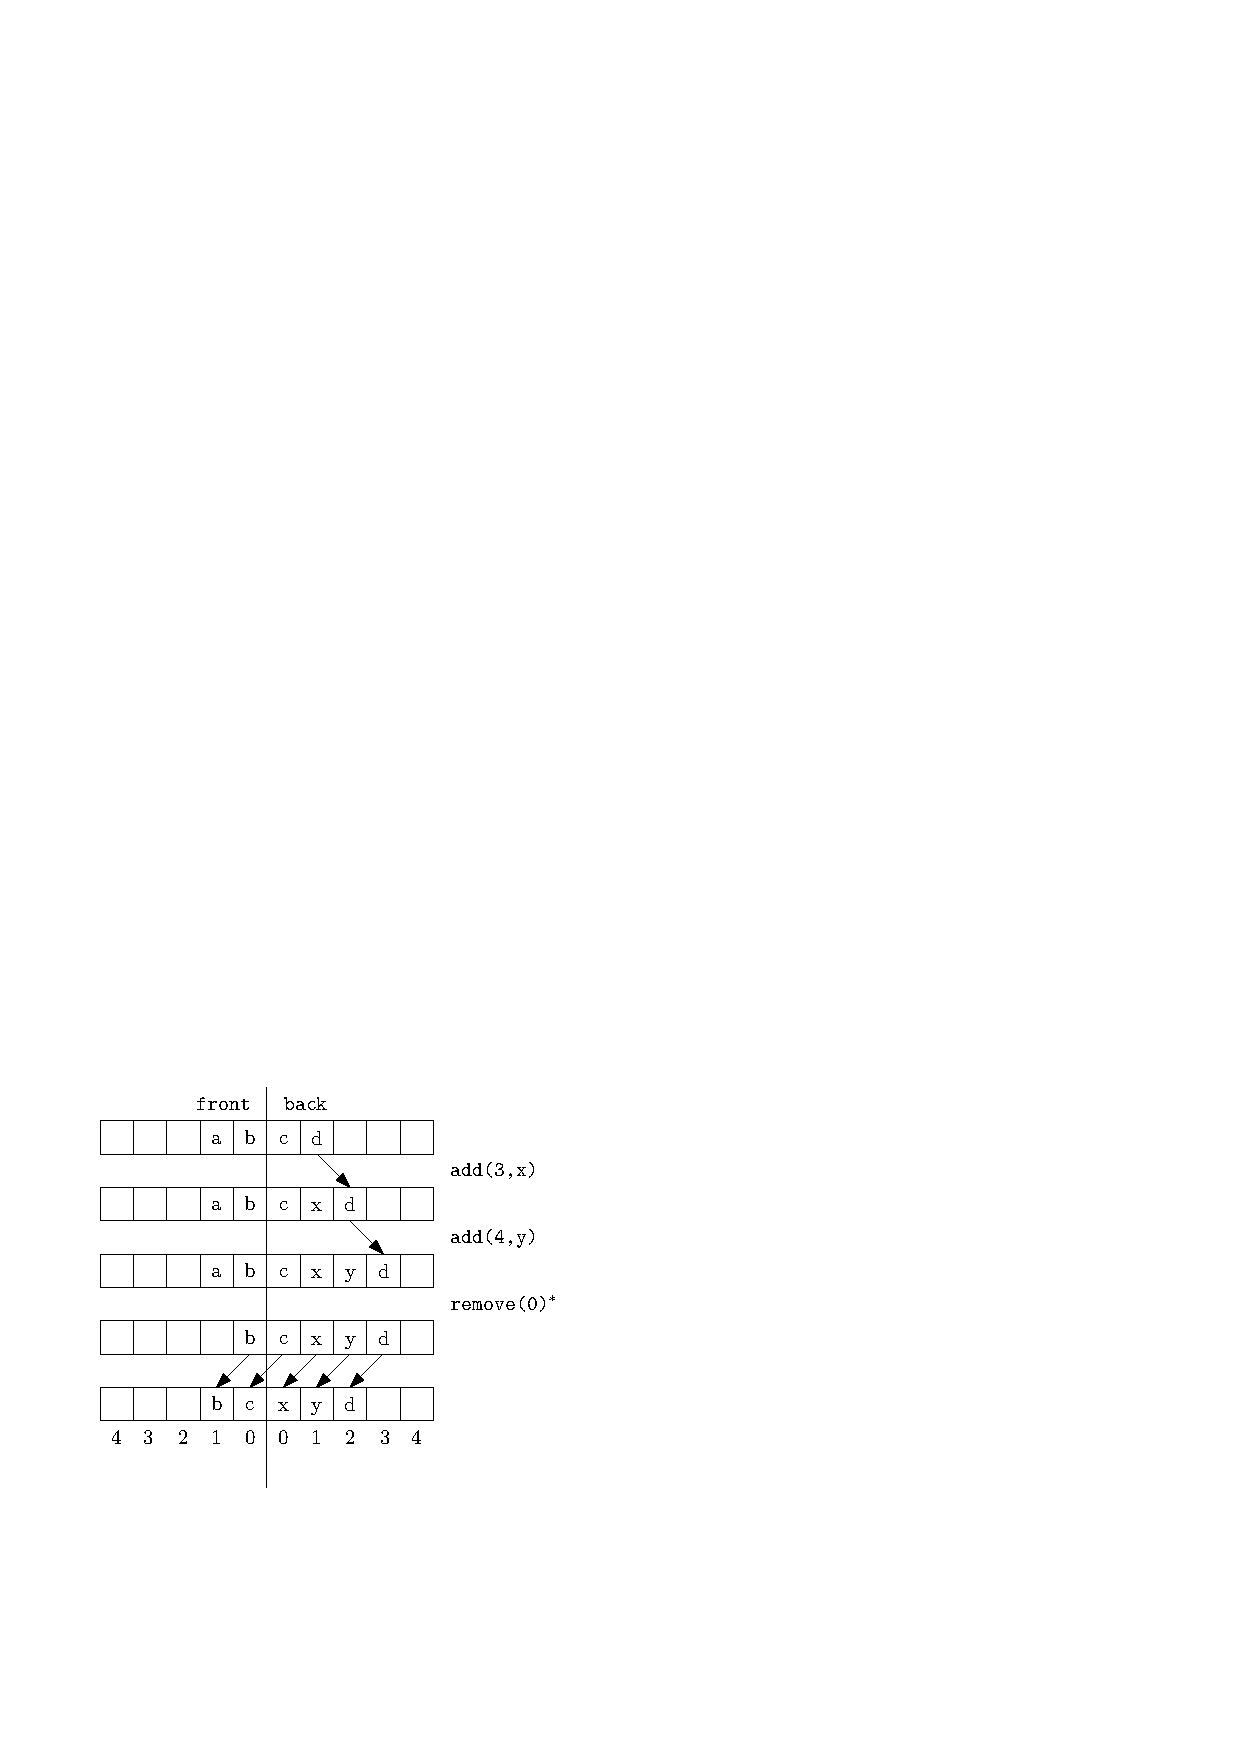
\includegraphics{figs/dualarraydeque}
  \end{center}
  \caption{A sequence of \mbox{\texttt{add({\color{var}i},{\color{var}x})}} and \mbox{\texttt{remove({\color{var}i})}} operation in a
  \mbox{\texttt{DualArrayDeque}}.  Arrows denote elements being copied.
  Operations that result in a rebalancing by \mbox{\texttt{rebalance()}} are marked with an asterisk.}
  \figlabel{dualarraydeque}
\end{figure}



\begin{Verbatim}[tabsize=2,frame=single,commandchars=\\@\$,label=\texttt{DualArrayDeque},labelposition=topline]
	@\color@var$void$ add(@\color@keyword$int$ @\color@var$i$, @\color@keyword$T$ @\color@var$x$) {
		@\color@keyword$if$ (@\color@var$i$ < @\color@var$front$.size()) { 
			@\color@var$front$.add(@\color@var$front$.size()-@\color@var$i$, @\color@var$x$);
		} @\color@keyword$else$ {
			@\color@var$back$.add(@\color@var$i$-@\color@var$front$.size(), @\color@var$x$);
		}
		balance();
	}
\end{Verbatim}

The \mbox{\texttt{add({\color{var}i},{\color{var}x})}} method performs rebalancing of the two \mbox{\texttt{ArrayStacks}}
\mbox{\texttt{{\color{var}front}}} and \mbox{\texttt{{\color{var}back}}}, by calling the \mbox{\texttt{balance()}} method.  The implementation
of \mbox{\texttt{balance()}} is described below, but for now it is sufficient to know
that \mbox{\texttt{balance()}} ensures that, unless $\mbox{\texttt{size()}}<2$, \mbox{\texttt{{\color{var}front}.size()}}
and \mbox{\texttt{{\color{var}back}.size()}} do not differ by more than a factor of 3.  In
particular, $3\mbox{\texttt{{\color{var}front}.size()}} \le \mbox{\texttt{{\color{var}back}.size()}}$ and $3\mbox{\texttt{{\color{var}back}.size()}}\le
\mbox{\texttt{{\color{var}front}.size()}}$.

Next we analyze the cost of \mbox{\texttt{add({\color{var}i},{\color{var}x})}}, ignoring the cost of the
\mbox{\texttt{balance()}} operation.  If $\mbox{\texttt{{\color{var}i}}}<\mbox{\texttt{{\color{var}front}.size()}}$, then this translates into $\mbox{\texttt{{\color{var}front}.add({\color{var}front}.size()-{\color{var}i}-1,{\color{var}x})}}$.  Since \mbox{\texttt{{\color{var}front}}} is an \mbox{\texttt{ArrayStack}}, the cost of this is 
\begin{equation}
  O(\mbox{\texttt{{\color{var}front}.size()}}-(\mbox{\texttt{{\color{var}front}.size()}}-\mbox{\texttt{{\color{var}i}}}-1)+1) = O(\mbox{\texttt{{\color{var}i}}}+1) \enspace .
  \eqlabel{das-front}
\end{equation}

On the other hand, if $\mbox{\texttt{{\color{var}i}}}\ge\mbox{\texttt{{\color{var}front}.size()}}$, then this translates into
$\mbox{\texttt{{\color{var}back}.add({\color{var}i}-{\color{var}front}.size(),{\color{var}x})}}$.  The cost of this is 
\begin{equation}
  O(\mbox{\texttt{{\color{var}back}.size()}}-(\mbox{\texttt{{\color{var}i}}}-\mbox{\texttt{{\color{var}front}.size()}})+1) = O(\mbox{\texttt{size()}}-\mbox{\texttt{{\color{var}i}}}+1)= O(\mbox{\texttt{{\color{var}n}}}-\mbox{\texttt{{\color{var}i}}}+1)\enspace .
  \eqlabel{das-back}
\end{equation}

Notice that the first case \eqref{das-front} occurs when $\mbox{\texttt{{\color{var}i}}}<\mbox{\texttt{{\color{var}n}}}/3$.
The second case \eqref{das-back} occurs when $\mbox{\texttt{{\color{var}i}}}>\mbox{\texttt{{\color{var}n}}}/3$.  When
$\mbox{\texttt{{\color{var}n}}}/3\le\mbox{\texttt{{\color{var}i}}}\le2\mbox{\texttt{{\color{var}n}}}/3$, we can't be sure whether the operation affects
\mbox{\texttt{{\color{var}front}}} or \mbox{\texttt{{\color{var}back}}}, but in either case, the operation takes $O(\mbox{\texttt{{\color{var}n}}})=O(\mbox{\texttt{{\color{var}i}}})$
time, since $\mbox{\texttt{{\color{var}i}}}\ge \mbox{\texttt{{\color{var}n}}}/3$.  Summarizing the situation, we have
\[
     \mbox{Running time of } \mbox{\texttt{add({\color{var}i},{\color{var}x})}} \le 
          \left\{\begin{array}{ll}
            O(1+ \mbox{\texttt{{\color{var}i}}}) & \mbox{if $\mbox{\texttt{{\color{var}i}}}< \mbox{\texttt{{\color{var}n}}}/3$} \\
            O(\mbox{\texttt{{\color{var}n}}}) & \mbox{if $\mbox{\texttt{{\color{var}n}}}/3 \le \mbox{\texttt{{\color{var}i}}} \le 2\mbox{\texttt{{\color{var}n}}}/3$} \\
            O(1+\mbox{\texttt{{\color{var}n}}}-\mbox{\texttt{{\color{var}i}}}) & \mbox{if $\mbox{\texttt{{\color{var}i}}} > 2\mbox{\texttt{{\color{var}n}}}/3$}
          \end{array}\right.
\]
Thus, the running time of \mbox{\texttt{add({\color{var}i},{\color{var}x})}} (ignoring the cost of the call to
\mbox{\texttt{balance()}}) is $O(1+\min\{\mbox{\texttt{{\color{var}i}}}, \mbox{\texttt{{\color{var}n}}}-\mbox{\texttt{{\color{var}i}}}\})$.

The \mbox{\texttt{remove({\color{var}i})}} operation, and its analysis, is similar to the \mbox{\texttt{add({\color{var}i},{\color{var}x})}}
operation.

\begin{Verbatim}[tabsize=2,frame=single,commandchars=\\@\$,label=\texttt{DualArrayDeque},labelposition=topline]
	@\color@keyword$T$ remove(@\color@keyword$int$ @\color@var$i$) {
		@\color@keyword$T$ @\color@var$x$;
		@\color@keyword$if$ (@\color@var$i$ < @\color@var$front$.size()) {
			@\color@var$x$ = @\color@var$front$.remove(@\color@var$front$.size()-@\color@var$i$-1);
		} @\color@keyword$else$ {
			@\color@var$x$ = @\color@var$back$.remove(@\color@var$i$-@\color@var$front$.size());
		}
		balance();
		@\color@var$return$ @\color@var$x$;
	}
\end{Verbatim}

\subsection{Balancing}

Finally, we study the \mbox{\texttt{balance()}} operation performed by \mbox{\texttt{add({\color{var}i},{\color{var}x})}}
and \mbox{\texttt{remove({\color{var}i})}}.  This operation is used to ensure that neither \mbox{\texttt{{\color{var}front}}}
nor \mbox{\texttt{{\color{var}back}}} gets too big (or too small).  It ensures that, unless there
are fewer than 2 elements, each of \mbox{\texttt{{\color{var}front}}} and \mbox{\texttt{{\color{var}back}}} contain at least
$\mbox{\texttt{{\color{var}n}}}/3$ elements. If this is not the case, then it moves elements between
them so that \mbox{\texttt{{\color{var}front}}} and \mbox{\texttt{{\color{var}back}}} contain exactly $\lfloor\mbox{\texttt{{\color{var}n}}}/2\rfloor$
elements and $\lceil\mbox{\texttt{{\color{var}n}}}/2\rceil$ elements, respectively.

\begin{Verbatim}[tabsize=2,frame=single,commandchars=\\@\$,label=\texttt{DualArrayDeque},labelposition=topline]
	@\color@var$void$ balance() {
		@\color@keyword$int$ @\color@var$n$ = size();
		@\color@keyword$if$ (3*@\color@var$front$.size() < @\color@var$back$.size()) {
			@\color@keyword$int$ @\color@var$s$ = @\color@var$n$/2 - @\color@var$front$.size();
			List<@\color@keyword$T$> @\color@var$l1$ = newStack();
			List<@\color@keyword$T$> @\color@var$l2$ = newStack();
			@\color@var$l1$.addAll(@\color@var$back$.subList(0,@\color@var$s$));
			Collections.reverse(@\color@var$l1$);
			@\color@var$l1$.addAll(@\color@var$front$);
			@\color@var$l2$.addAll(@\color@var$back$.subList(@\color@var$s$, @\color@var$back$.size()));
			@\color@var$front$ = @\color@var$l1$;
			@\color@var$back$ = @\color@var$l2$;
		} @\color@keyword$else$ @\color@keyword$if$ (3*@\color@var$back$.size() < @\color@var$front$.size()) {
			@\color@keyword$int$ @\color@var$s$ = @\color@var$front$.size() - @\color@var$n$/2;
			List<@\color@keyword$T$> @\color@var$l1$ = newStack();
			List<@\color@keyword$T$> @\color@var$l2$ = newStack();
			@\color@var$l1$.addAll(@\color@var$front$.subList(@\color@var$s$, @\color@var$front$.size()));
			@\color@var$l2$.addAll(@\color@var$front$.subList(0, @\color@var$s$));
			Collections.reverse(@\color@var$l2$);
			@\color@var$l2$.addAll(@\color@var$back$);
			@\color@var$front$ = @\color@var$l1$;
			@\color@var$back$ = @\color@var$l2$;
		}
	}
\end{Verbatim}

There is not much to analyze.  If the \mbox{\texttt{balance()}} operation does
do rebalancing, then it moves $\Theta(\mbox{\texttt{{\color{var}n}}})$ elements and this takes
$O(\mbox{\texttt{{\color{var}n}}})$ time. This is bad, since \mbox{\texttt{balance()}} is called with each call to
\mbox{\texttt{add({\color{var}i},{\color{var}x})}} and \mbox{\texttt{remove({\color{var}i})}}.  However, the following theorem shows that,
on average, \mbox{\texttt{balance()}} only does a constant amount of work per operation

\begin{lem}\lemlabel{dualarraydeque-amortized}
  If an empty \mbox{\texttt{DualArrayDeque}} is created and any sequence of $m\ge 1$ calls
  to \mbox{\texttt{add({\color{var}i},{\color{var}x})}} and \mbox{\texttt{remove({\color{var}i})}} are performed, then the total cost of all work
  done during all calls to \mbox{\texttt{balance()}} is $O(m)$.
\end{lem}

\begin{proof}
  We will show that, if \mbox{\texttt{balance()}} is forced to shift elements,
  then the number of \mbox{\texttt{add({\color{var}i},{\color{var}x})}} and \mbox{\texttt{remove({\color{var}i})}} operations since the
  last time \mbox{\texttt{balance()}} shifted any elements was at least $\mbox{\texttt{{\color{var}n}}}/2-1$.
  As in the proof of \lemref{arraystack-amortized}, this is sufficient
  to prove that the total work done by \mbox{\texttt{balance()}} is $O(m)$.

  We will perform our analysis using the \emph{potential method}.
  Define the \emph{potential} of the \mbox{\texttt{DualArrayDeque}} as
  \[  \Phi = |\mbox{\texttt{{\color{var}front}.size()}} - \mbox{\texttt{{\color{var}back}.size()}}| \enspace . \]
  The interesting thing about this potential is that a call to \mbox{\texttt{add({\color{var}i},{\color{var}x})}}
  or \mbox{\texttt{remove({\color{var}i})}} that does not do any balancing can increase the potential
  by at most 1.

  Observe that, immediately after a call to \mbox{\texttt{balance()}} that shifts
  elements, the potential, $\Phi_0$, is at most 1, since
  \[ \Phi_0 = \left|\lfloor\mbox{\texttt{{\color{var}n}}}/2\rfloor-\lceil\mbox{\texttt{{\color{var}n}}}/2\rceil\right|\le 1  \enspace .\]

  Now, consider the situation immediately before a call to \mbox{\texttt{balance()}} that
  shifts elements, and suppose, without loss of generality that \mbox{\texttt{balance()}}
  is shifting elements because $3\mbox{\texttt{{\color{var}front}.size()}} < \mbox{\texttt{{\color{var}back}.size()}}$.
  Notice that, in this case,
  \begin{eqnarray*}
   \mbox{\texttt{{\color{var}n}}} & = & \mbox{\texttt{{\color{var}front}.size()}}+\mbox{\texttt{{\color{var}back}.size()}} \\
       & \le & \mbox{\texttt{{\color{var}back}.size()/3}}+\mbox{\texttt{{\color{var}back}.size()}} \\
       & = & \frac{4}{3}\mbox{\texttt{{\color{var}back}.size()}}
  \end{eqnarray*}
  Furthermore, the potential at this point in time is
  \begin{eqnarray*}
  \Phi_1 & = & \mbox{\texttt{{\color{var}back}.size()}} - \mbox{\texttt{{\color{var}front}.size()}} \\
      &>& \mbox{\texttt{{\color{var}back}.size()}} - \mbox{\texttt{{\color{var}back}.size()/3}} \\
      &=& \frac{2}{3}\mbox{\texttt{{\color{var}back}.size()}} \\
      &\ge& \frac{3}{4}\times\frac{2}{3}\mbox{\texttt{{\color{var}n}}} \\
      &=& \mbox{\texttt{{\color{var}n}}}/2
  \end{eqnarray*}
  Therefore, the number of calls to \mbox{\texttt{add({\color{var}i},{\color{var}x})}} or \mbox{\texttt{remove({\color{var}i})}} since
  the last time \mbox{\texttt{balance()}} shifted elements is at least $\Phi_1-\Phi_0
  \ge \mbox{\texttt{{\color{var}n}}}/2-1$. This completes the proof.
\end{proof}

\subsection{Summary}

The following theorem summarizes the performance of a \mbox{\texttt{DualArrayStack}}

\begin{thm}\thmlabel{dualarraydeque}
  A \mbox{\texttt{DualArrayDeque}} implements the \mbox{\texttt{List}} interface.  Ignoring the
  cost of calls to \mbox{\texttt{resize()}} and \mbox{\texttt{balance()}}, an \mbox{\texttt{DualArrayDeque}}
  supports the operations
  \begin{itemize}
    \item \mbox{\texttt{get({\color{var}i})}} and \mbox{\texttt{set({\color{var}i},{\color{var}x})}} in $O(1)$ time per operation; and
    \item \mbox{\texttt{add({\color{var}i},{\color{var}x})}} and \mbox{\texttt{remove({\color{var}i})}} in $O(1+\min\{\mbox{\texttt{{\color{var}i}}},\mbox{\texttt{{\color{var}n}}}-\mbox{\texttt{{\color{var}i}}}\})$ time
          per operation.
  \end{itemize}
  Furthermore, beginning with an empty \mbox{\texttt{DualArrayDeque}}, any sequence of $m$
  \mbox{\texttt{add({\color{var}i},{\color{var}x})}} and \mbox{\texttt{remove({\color{var}i})}} operations results in a total of $O(m)$
  work during all calls to \mbox{\texttt{resize()}} and \mbox{\texttt{balance()}}.
\end{thm}


\section{\mbox{\texttt{RootishArrayStack}}: A Space-Efficient Array Stack}

One of the drawbacks of all previous data structures in this chapter
is that, because they store their data in one or two arrays, and they
don't want to resize these arrays too often, the arrays are frequently
not very full.  For example, immediately after a \mbox{\texttt{resize()}} operation on
an \mbox{\texttt{ArrayStack}}, the backing array \mbox{\texttt{{\color{var}a}}} is only half full.  Even worse,
there are times when only $1/3$ of \mbox{\texttt{{\color{var}a}}} contains data.

In this section, we discuss a data structure, the \mbox{\texttt{RootishArrayStack}},
that addresses this problem of wasted space.  The \mbox{\texttt{RootishArrayStack}}
stores \mbox{\texttt{{\color{var}n}}} elements using $O(\sqrt{\mbox{\texttt{{\color{var}n}}}})$ arrays.  In these arrays, at
most $O(\sqrt{\mbox{\texttt{{\color{var}n}}}})$ array locations are unused.  All remaining array
locations are used to store data.  Therefore, these data structures waste
at most $O(\sqrt{\mbox{\texttt{{\color{var}n}}}})$ space when storing \mbox{\texttt{{\color{var}n}}} elements.

A \mbox{\texttt{RootishArrayStack}} stores its elements in a list of \mbox{\texttt{{\color{var}r}}}
arrays called \emph{blocks} that are numbered $0,1,\ldots,\mbox{\texttt{{\color{var}r}}}-1$.
See \figref{rootisharraystack}.  Block $b$ contains $b+1$ elements.
Therefore, all \mbox{\texttt{{\color{var}r}}} blocks contain a total of
\[
  1+ 2+ 3+\cdots +\mbox{\texttt{{\color{var}r}}} = \mbox{\texttt{{\color{var}r}}}(\mbox{\texttt{{\color{var}r}}}+1)/2
\]
elements.  The above formula (allegedly discovered by the Gau\ss\ at
the age of 9) can be obtained as shown in \figref{gauss}.

\begin{figure}
  \begin{center}
    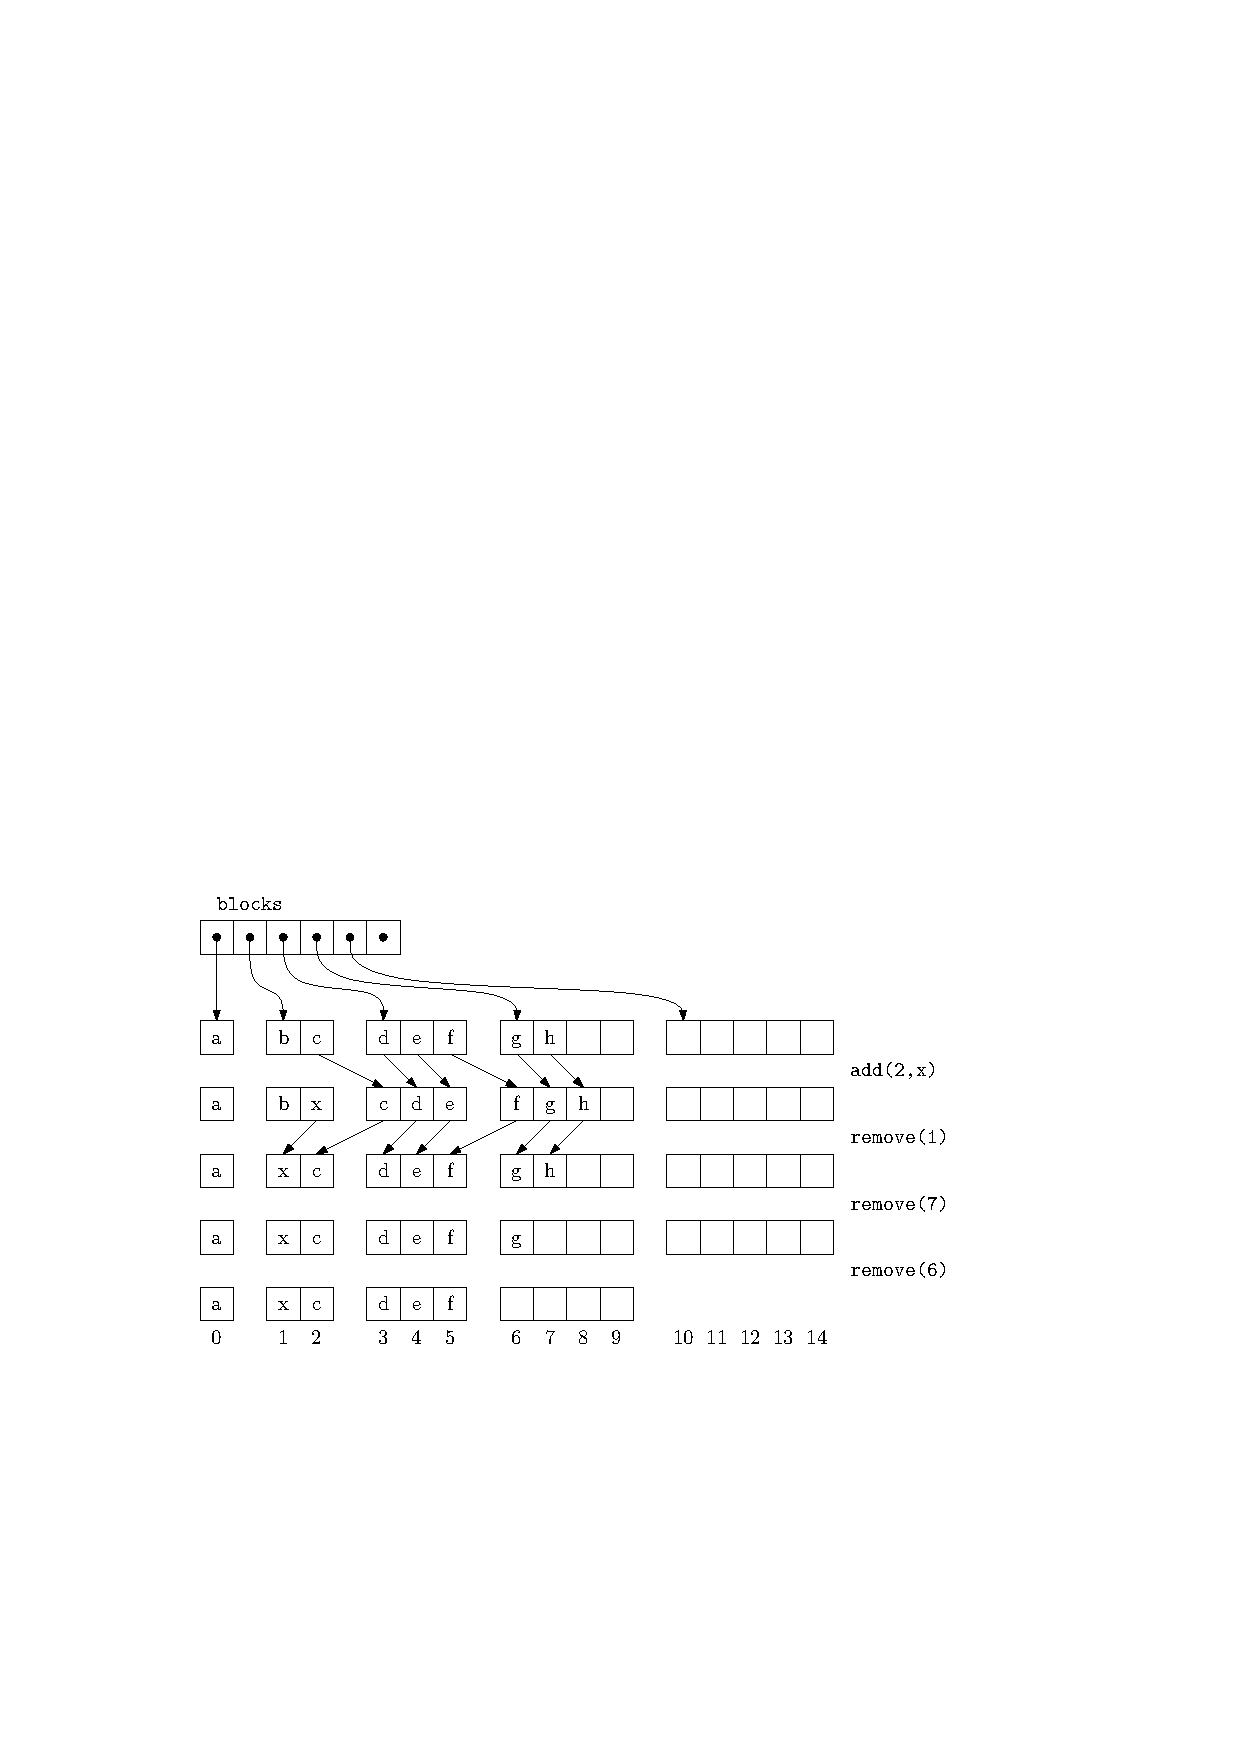
\includegraphics{figs/rootisharraystack}
  \end{center}
  \caption{A sequence of \mbox{\texttt{add({\color{var}i},{\color{var}x})}} and \mbox{\texttt{remove({\color{var}i})}} operation in a
  \mbox{\texttt{RootishArrayStack}}.  Arrows denote elements being copied. }
  \figlabel{rootisharraystack}
\end{figure}

\begin{Verbatim}[tabsize=2,frame=single,commandchars=\\@\$,label=\texttt{RootishArrayStack},labelposition=topline]
	List<@\color@keyword$T$[]> @\color@var$blocks$;
	@\color@keyword$int$ @\color@var$n$;
\end{Verbatim}

\begin{figure}
  \begin{center}
    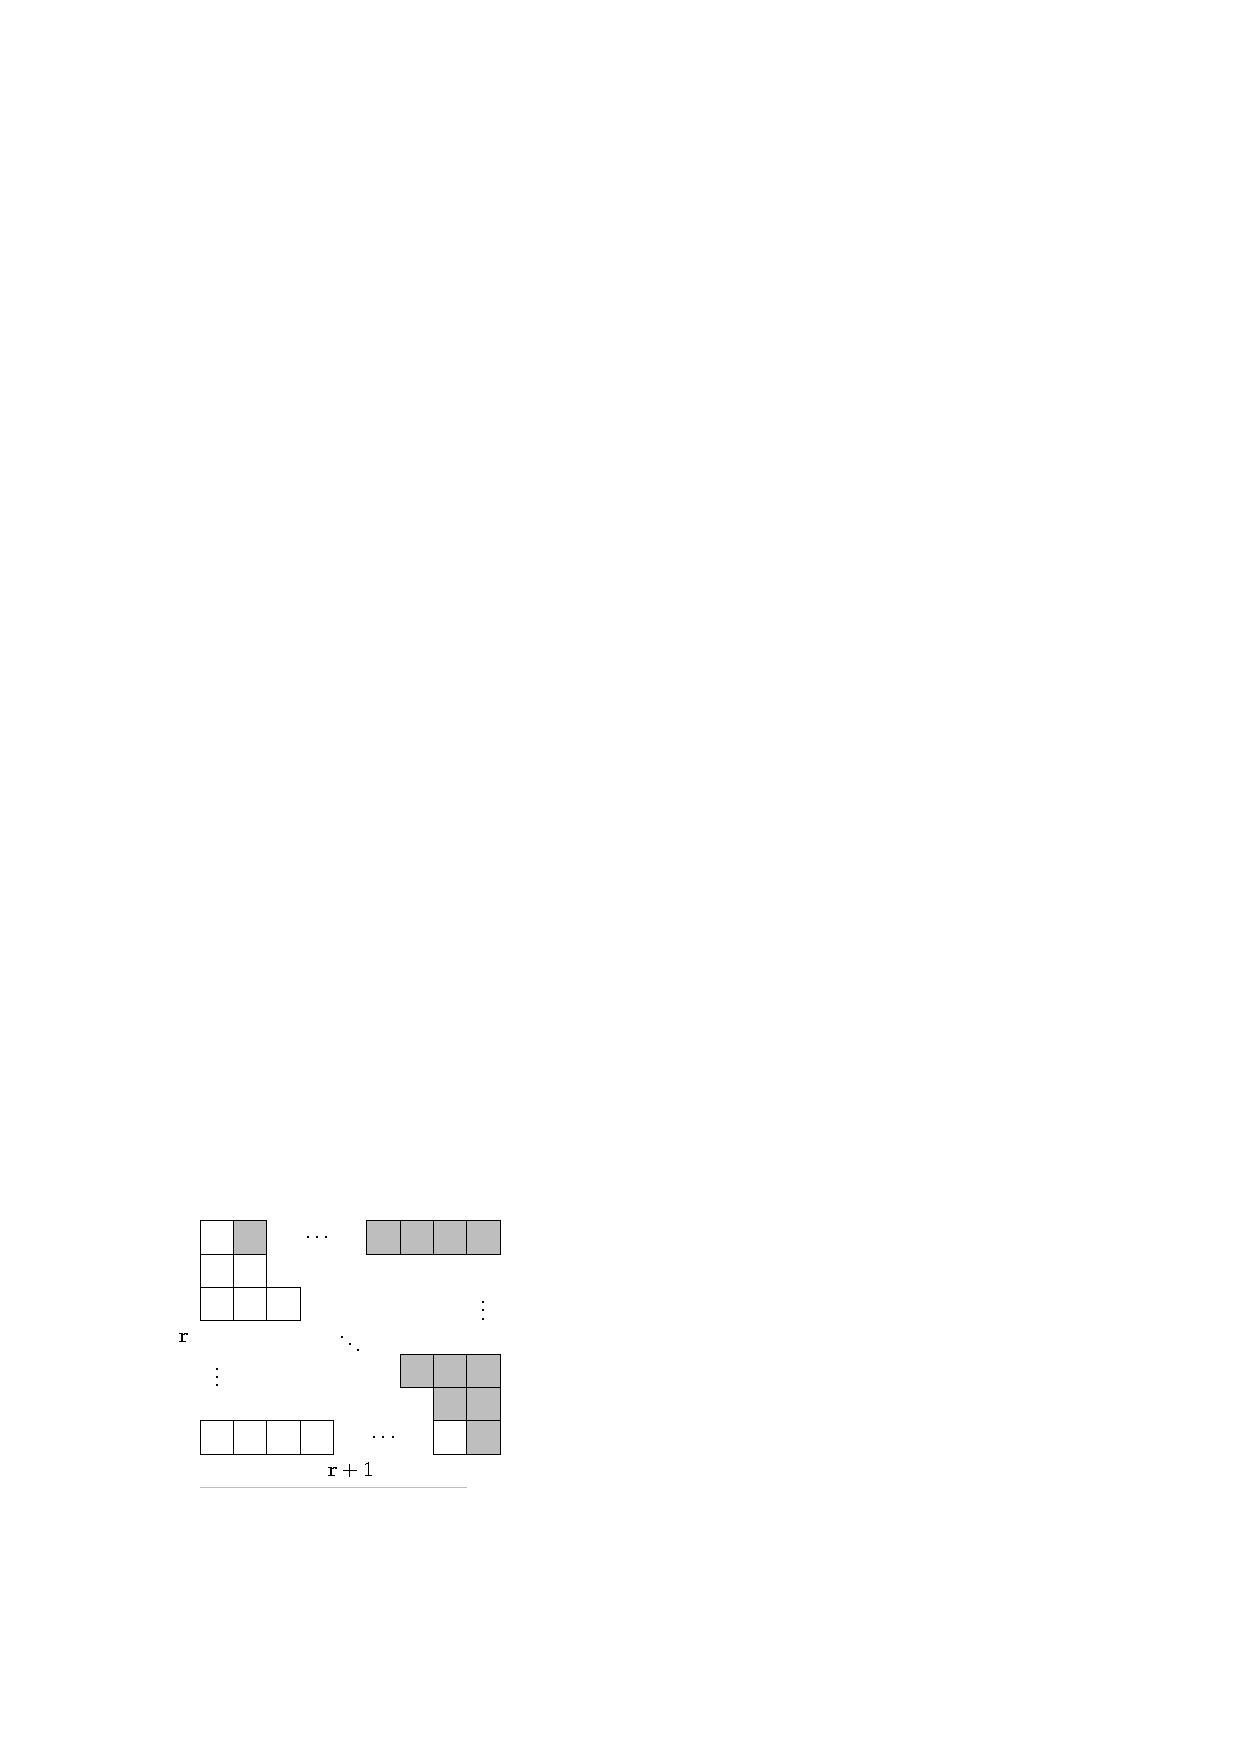
\includegraphics{figs/gauss}
  \end{center}
  \caption{The number of white squares is $1+2+3+\cdots+\mbox{\texttt{{\color{var}r}}}$.  The number of
  shaded squares is the same.  Together the white and shaded squares make a
  rectangle consisting of $\mbox{\texttt{{\color{var}r}}}(\mbox{\texttt{{\color{var}r}}}+1)$ squares.}
  \figlabel{gauss}
\end{figure}

The elements of the list are layed out in the blocks as we might expect.
The list element with index 0 is stored in block 0,  the elements with
list indices 1 and 2 are stored in block 1, the elements with list
indices 3, 4, and 5 are stored in block 2, and so on.  The main problem
we have to address is that of determining, given an index $\mbox{\texttt{{\color{var}i}}}$, which
block contains \mbox{\texttt{{\color{var}i}}} as well as the index of \mbox{\texttt{{\color{var}i}}} within its block.

Determining the index of \mbox{\texttt{{\color{var}i}}} within its block turns out to be easy. If
index \mbox{\texttt{{\color{var}i}}} is in block \mbox{\texttt{{\color{var}b}}}, then the number of elements in blocks
$0,\ldots,\mbox{\texttt{{\color{var}b}}}-1$ is $\mbox{\texttt{{\color{var}b}}}(\mbox{\texttt{{\color{var}b}}}+1)/2$.  Therefore, \mbox{\texttt{{\color{var}i}}} is stored at location
\[
     \mbox{\texttt{{\color{var}j}}} = \mbox{\texttt{{\color{var}i}}} - \mbox{\texttt{{\color{var}b}}}(\mbox{\texttt{{\color{var}b}}}+1)/2
\]
within block \mbox{\texttt{{\color{var}b}}}.  Somewhat more challenging is the problem of determining
the value of \mbox{\texttt{{\color{var}b}}}.  The number of elements that have indices less than
or equal to \mbox{\texttt{{\color{var}i}}} is $\mbox{\texttt{{\color{var}i}}}+1$.  On the other hand, the number of elements
in blocks 0,\ldots,b is $(\mbox{\texttt{{\color{var}b}}}+1)(\mbox{\texttt{{\color{var}b}}}+2)/2$.  Therefore, \mbox{\texttt{{\color{var}b}}} is smallest
integer such that
\[
    (\mbox{\texttt{{\color{var}b}}}+1)(\mbox{\texttt{{\color{var}b}}}+2)/2 \ge \mbox{\texttt{{\color{var}i}}}+1 \enspace .
\]
We can rewrite this equation as
\[
    \mbox{\texttt{{\color{var}b}}}^2 + 3\mbox{\texttt{{\color{var}b}}} - 2\mbox{\texttt{{\color{var}i}}} \ge  0 \enspace .
\]
The corresponding quadratic equation $\mbox{\texttt{{\color{var}b}}}^2 + 3\mbox{\texttt{{\color{var}b}}} - 2\mbox{\texttt{{\color{var}i}}} =  0$ has two
solutions: $\mbox{\texttt{{\color{var}b}}}=(-3 + \sqrt{9+8\mbox{\texttt{{\color{var}i}}}}) / 2$ and $\mbox{\texttt{{\color{var}b}}}=(-3 - \sqrt{9+8\mbox{\texttt{{\color{var}i}}}}) / 2$.
The second solution makes no sense in our application since it always
gives a negative value. Therefore, we obtain the solution $b = (-3 +
\sqrt{9+8i}) / 2$.  In general, this solution is not an integer, but
going back to our inequality, we want the smallest integer $b$ such that 
$b \ge (-3 + \sqrt{9+8i}) / 2$.  This is simply
\[
   b = \left\lceil(-3 + \sqrt{9+8i}) / 2\right\rceil \enspace .
\]

\begin{Verbatim}[tabsize=2,frame=single,commandchars=\\@\$,label=\texttt{RootishArrayStack},labelposition=topline]
	 @\color@keyword$int$ i2b(@\color@keyword$int$ @\color@var$i$) {
		@\color@keyword$double$ @\color@var$db$ = (-3.0 + Math.sqrt(9 + 8*@\color@var$i$)) / 2.0;
		@\color@keyword$int$ @\color@var$b$ = (@\color@keyword$int$)Math.ceil(@\color@var$db$);
		@\color@var$return$ @\color@var$b$; 
	}
\end{Verbatim}

With this out of the way, the \mbox{\texttt{get({\color{var}i})}} and \mbox{\texttt{set({\color{var}i},{\color{var}x})}} methods are straightforward.  We first compute the appropriate block \mbox{\texttt{{\color{var}b}}} and the appropriate index \mbox{\texttt{{\color{var}j}}} within the block and then perform the appropriate operation:

\begin{Verbatim}[tabsize=2,frame=single,commandchars=\\@\$,label=\texttt{RootishArrayStack},labelposition=topline]
	@\color@keyword$T$ get(@\color@keyword$int$ @\color@var$i$) {
		@\color@keyword$if$ (@\color@var$i$ < 0 || @\color@var$i$ > @\color@var$n$ - 1) @\color@keyword$throw$ @\color@keyword$new$ IndexOutOfBoundsException();
		@\color@keyword$int$ @\color@var$b$ = i2b(@\color@var$i$);
		@\color@keyword$int$ @\color@var$j$ = @\color@var$i$ - @\color@var$b$*(@\color@var$b$+1)/2;
		@\color@var$return$ @\color@var$blocks$.get(@\color@var$b$)[@\color@var$j$];
	}
	@\color@keyword$T$ set(@\color@keyword$int$ @\color@var$i$, @\color@keyword$T$ @\color@var$x$) {
		@\color@keyword$if$ (@\color@var$i$ < 0 || @\color@var$i$ > @\color@var$n$ - 1) @\color@keyword$throw$ @\color@keyword$new$ IndexOutOfBoundsException();
		@\color@keyword$int$ @\color@var$b$ = i2b(@\color@var$i$);
		@\color@keyword$int$ @\color@var$j$ = @\color@var$i$ - @\color@var$b$*(@\color@var$b$+1)/2;
		@\color@keyword$T$ @\color@var$y$ = @\color@var$blocks$.get(@\color@var$b$)[@\color@var$j$];
		@\color@var$blocks$.get(@\color@var$b$)[@\color@var$j$] = @\color@var$x$;
		@\color@var$return$ @\color@var$y$;
	}
\end{Verbatim}

If we use any of the data structures in this chapter for representing the \mbox{\texttt{{\color{var}blocks}}} list, then \mbox{\texttt{get({\color{var}i})}} and \mbox{\texttt{set({\color{var}i},{\color{var}x})}} will each run in constant time.

The \mbox{\texttt{add({\color{var}i},{\color{var}x})}} method will, by now, look familiar.  We first check if
our data structure is full, by checking if the number of blocks \mbox{\texttt{{\color{var}r}}}
is such that that $\mbox{\texttt{{\color{var}r}}}(\mbox{\texttt{{\color{var}r}}}+1) = \mbox{\texttt{{\color{var}n}}}$ and, if so, we call \mbox{\texttt{grow()}}
to add another block.  With this done, we shift elements with indices
$\mbox{\texttt{{\color{var}i}}},\ldots,\mbox{\texttt{{\color{var}n}}}-1$ to the right by one position to make room for the
new element with index \mbox{\texttt{{\color{var}i}}}:

\begin{Verbatim}[tabsize=2,frame=single,commandchars=\\@\$,label=\texttt{RootishArrayStack},labelposition=topline]
	@\color@var$void$ add(@\color@keyword$int$ @\color@var$i$, @\color@keyword$T$ @\color@var$x$) {
		@\color@keyword$if$ (@\color@var$i$ < 0 || @\color@var$i$ > @\color@var$n$) @\color@keyword$throw$ @\color@keyword$new$ IndexOutOfBoundsException();
		@\color@keyword$int$ @\color@var$r$ = @\color@var$blocks$.size();
		@\color@keyword$if$ (@\color@var$r$*(@\color@var$r$+1)/2 < @\color@var$n$ + 1) grow();
		@\color@var$n$++;
		@\color@keyword$for$ (@\color@keyword$int$ @\color@var$j$ = @\color@var$n$-1; @\color@var$j$ > @\color@var$i$; @\color@var$j$--)
			set(@\color@var$j$, get(@\color@var$j$-1));
		set(@\color@var$i$, @\color@var$x$);
	}
\end{Verbatim}

The \mbox{\texttt{grow()}} method does what we expect. It adds a new block:

\begin{Verbatim}[tabsize=2,frame=single,commandchars=\\@\$,label=\texttt{RootishArrayStack},labelposition=topline]
	@\color@var$void$ grow() {
		@\color@var$blocks$.add(newArray(@\color@var$blocks$.size()+1));
	}
\end{Verbatim}

Ignoring the cost of the \mbox{\texttt{grow()}} operation, the cost of an \mbox{\texttt{add({\color{var}i},{\color{var}x})}}
operation is dominated by the cost of shifting and is therefore
$O(1+\mbox{\texttt{{\color{var}n}}}-\mbox{\texttt{{\color{var}i}}})$, just like an \mbox{\texttt{ArrayStack}}.

The \mbox{\texttt{remove({\color{var}i})}} operation is similar to \mbox{\texttt{add({\color{var}i},{\color{var}x})}}.  It shifts the
elements with indices $\mbox{\texttt{{\color{var}i}}}+1,\ldots,\mbox{\texttt{{\color{var}n}}}$ left by one position and then,
if there is more than one empty block, it calls the \mbox{\texttt{shrink()}} method
to remove all but one of the unused blocks:

\begin{Verbatim}[tabsize=2,frame=single,commandchars=\\@\$,label=\texttt{RootishArrayStack},labelposition=topline]
	@\color@keyword$T$ remove(@\color@keyword$int$ @\color@var$i$) {
		@\color@keyword$if$ (@\color@var$i$ < 0 || @\color@var$i$ > @\color@var$n$ - 1) @\color@keyword$throw$ @\color@keyword$new$ IndexOutOfBoundsException();
		@\color@keyword$T$ @\color@var$x$ = get(@\color@var$i$);
		@\color@keyword$for$ (@\color@keyword$int$ @\color@var$j$ = @\color@var$i$; @\color@var$j$ < @\color@var$n$-1; @\color@var$j$++)
			set(@\color@var$j$, get(@\color@var$j$+1));
		@\color@var$n$--;
		@\color@keyword$int$ @\color@var$r$ = @\color@var$blocks$.size();
		@\color@keyword$if$ ((@\color@var$r$-2)*(@\color@var$r$-1)/2 >= @\color@var$n$)	shrink();
		@\color@var$return$ @\color@var$x$;
	}
\end{Verbatim}
\begin{Verbatim}[tabsize=2,frame=single,commandchars=\\@\$,label=\texttt{RootishArrayStack},labelposition=topline]
	@\color@var$void$ shrink() {
		@\color@keyword$int$ @\color@var$r$ = @\color@var$blocks$.size();
		@\color@keyword$while$ (@\color@var$r$ > 0 && (@\color@var$r$-2)*(@\color@var$r$-1)/2 >= @\color@var$n$) {
			@\color@var$blocks$.remove(@\color@var$blocks$.size()-1);
			@\color@var$r$--;
		}
	}
\end{Verbatim}

Once again, ignoring the cost of the \mbox{\texttt{shrink()}} operation, the cost of
a \mbox{\texttt{remove({\color{var}i})}} operation is dominated by the cost of shifting  and is
therefore $O(\mbox{\texttt{{\color{var}n}}}-\mbox{\texttt{{\color{var}i}}})$

\subsection{Analysis of Growing and Shrinking}

The analysis of \mbox{\texttt{add({\color{var}i},{\color{var}x})}} and \mbox{\texttt{remove({\color{var}i})}} does not account for the cost
of \mbox{\texttt{grow()}} and \mbox{\texttt{shrink()}}.  Note that, unlike the \mbox{\texttt{ArrayStack.resize()}}
operation, \mbox{\texttt{grow()}} and \mbox{\texttt{shrink()}} do not do any copying of data.
They only allocate or free an array of size \mbox{\texttt{{\color{var}r}}}.  In some
environments, this takes only constant time, while in others, it may
require $\Theta(\mbox{\texttt{{\color{var}r}}}))$ time.

We note that, immediately after a call to \mbox{\texttt{grow()}} or \mbox{\texttt{shrink()}}, the
situation is clear. The final block is completely empty and all other
blocks are completely full.  Another call to \mbox{\texttt{grow()}} or \mbox{\texttt{shrink()}} will
not happen until at least $\mbox{\texttt{{\color{var}r}}}-1$ elements have been added or removed.
Therefore, even if \mbox{\texttt{grow()}} and \mbox{\texttt{shrink()}} take $O(\mbox{\texttt{{\color{var}r}}})$ time, this
cost can be amortized over at least $\mbox{\texttt{{\color{var}r}}}-1$ \mbox{\texttt{add({\color{var}i},{\color{var}x})}} or \mbox{\texttt{remove({\color{var}i})}}
operations, so that the amortized cost of \mbox{\texttt{grow()}} and \mbox{\texttt{shrink()}} is
$O(1)$ per operation.

\subsection{Space Usage}

Next, we analyze the amount of extra space used by a \mbox{\texttt{RootishArrayStack}}.
In particular, we want to count any space used by a \mbox{\texttt{RootishArrayStack}} that is not an array element currently used to hold a list element.  We call all such space \emph{wasted space}.

The \mbox{\texttt{remove({\color{var}i})}} operation ensures that a \mbox{\texttt{RootishArrayStack}} never has
more than 2 blocks that are not completely full.  The number of blocks,
\mbox{\texttt{{\color{var}r}}}, used by a \mbox{\texttt{RootishArrayStack}} that stores \mbox{\texttt{{\color{var}n}}} elements therefore
satisfies
\[
    (\mbox{\texttt{{\color{var}r}}}-2)(\mbox{\texttt{{\color{var}r}}}-1) \le \mbox{\texttt{{\color{var}n}}}
\]
Again, using the quadratic equation on this gives
\[
   \mbox{\texttt{{\color{var}r}}} \le (3+\sqrt{1+4\mbox{\texttt{{\color{var}n}}}})/2 = O(\sqrt{\mbox{\texttt{{\color{var}n}}}})
\]
The last two blocks have sizes \mbox{\texttt{{\color{var}r}}} and \mbox{\texttt{{\color{var}r}-1}}, so the space wasted by these
two blocks is at most $2\mbox{\texttt{{\color{var}r}}} = O(\sqrt{\mbox{\texttt{{\color{var}n}}}})$.  If we store the blocks
in (for example) an \mbox{\texttt{ArrayList}}, then the amount of space wasted by the
\mbox{\texttt{List}} that stores those \mbox{\texttt{{\color{var}r}}} blocks is also $O(\mbox{\texttt{{\color{var}r}}})=O(\sqrt{\mbox{\texttt{{\color{var}n}}}})$.  The
other space for storing \mbox{\texttt{{\color{var}n}}} and other accounting information is $O(1)$.
Therefore, the total amount of wasted space in a \mbox{\texttt{RootishArrayStack}}
is $O(\sqrt{\mbox{\texttt{{\color{var}n}}}})$.

Next, we argue that this is optimal for any data structure that starts out
empty and can support the addition of one item at a time. More precisely,
we will show that, at some point during the addition of \mbox{\texttt{{\color{var}n}}} items, the
data structure has at least $\sqrt{\mbox{\texttt{{\color{var}n}}}}$ wasted space (though it may be
only for a moment).

Suppose we start with an empty data structure and we add \mbox{\texttt{{\color{var}n}}} items
one at a time.  At the end of this process, all \mbox{\texttt{{\color{var}n}}} items are stored
in the structure and they are distributed among a collection of \mbox{\texttt{{\color{var}r}}}
memory blocks.  If $\mbox{\texttt{{\color{var}r}}}\ge \sqrt{\mbox{\texttt{{\color{var}n}}}}$, then the data structure must be
using \mbox{\texttt{{\color{var}r}}} pointers (or references) to keep track of these \mbox{\texttt{{\color{var}r}}} blocks,
and this is wasted space.  On the other hand, if $\mbox{\texttt{{\color{var}r}}} < \sqrt{\mbox{\texttt{{\color{var}n}}}}$
then, by the pigeonhole principle, some block must have size at least
$\mbox{\texttt{{\color{var}n}}}/\mbox{\texttt{{\color{var}r}}} > \sqrt{\mbox{\texttt{{\color{var}n}}}}$.  Consider the moment at which this block was
first allocated.  Immediately after it was allocated, this block was
empty, and was therefore wasting $\sqrt{\mbox{\texttt{{\color{var}n}}}}$ space.  Therefore, at some
point in time during the insertion of \mbox{\texttt{{\color{var}n}}} elements, the data structure was
wasting $O(\sqrt{\mbox{\texttt{{\color{var}n}}}})$ space.

\subsection{Summary}

The following theorem summarizes the performance of the \mbox{\texttt{RootishArrayStack}}
data structure:

\begin{thm}\thmlabel{rootisharraystack}
  A \mbox{\texttt{RootishArrayStack}} implements the \mbox{\texttt{List}} interface.  Ignoring the cost of
  calls to \mbox{\texttt{grow()}} and \mbox{\texttt{shrink()}}, a \mbox{\texttt{RootishArrayStack}} supports the operations
  \begin{itemize}
    \item \mbox{\texttt{get({\color{var}i})}} and \mbox{\texttt{set({\color{var}i},{\color{var}x})}} in $O(1)$ time per operation; and
    \item \mbox{\texttt{add({\color{var}i},{\color{var}x})}} and \mbox{\texttt{remove({\color{var}i})}} in $O(1+\mbox{\texttt{{\color{var}n}}}-\mbox{\texttt{{\color{var}i}}})$ time per operation.
  \end{itemize}
  Furthermore, beginning with an empty \mbox{\texttt{RootishArrayStack}}, any sequence of $m$
  \mbox{\texttt{add({\color{var}i},{\color{var}x})}} and \mbox{\texttt{remove({\color{var}i})}} operations results in a total of $O(m)$
  work during all calls to \mbox{\texttt{grow()}} and \mbox{\texttt{shrink()}}.

  The space (measured in words)\footnote{Recall \secref{model} for a
  discussion of how memory is measured.} used by a \mbox{\texttt{RootishArrayStack}}
  that stores \mbox{\texttt{{\color{var}n}}} elements is $\mbox{\texttt{{\color{var}n}}} +O(\sqrt{\mbox{\texttt{{\color{var}n}}}})$.
\end{thm}

\section{Exercises}


\begin{enumerate}
\item The \mbox{\texttt{List}} method \mbox{\texttt{addAll({\color{var}i},{\color{var}c})}} inserts all elements of the
\mbox{\texttt{Collection}} \mbox{\texttt{{\color{var}c}}} into the list at position \mbox{\texttt{{\color{var}i}}}.  (The \mbox{\texttt{add({\color{var}i},{\color{var}x})}} method is a special case where $\mbox{\texttt{{\color{var}c}}}=\{\mbox{\texttt{{\color{var}x}}}\}$.)  Explain why, for the data structures in this chapter, it is not efficient to implement \mbox{\texttt{addAll({\color{var}i},{\color{var}c})}} by repeated calls to \mbox{\texttt{add({\color{var}i},{\color{var}x})}}.  Describe a more efficient implementation.

\item Design and implement a \mbox{\texttt{Treque}} (triple-ended queue). This is a \mbox{\texttt{List}} implementation in which \mbox{\texttt{get({\color{var}i})}} and \mbox{\texttt{set({\color{var}i},{\color{var}x})}} run in constant time and \mbox{\texttt{add({\color{var}i},{\color{var}x})}} and \mbox{\texttt{remove({\color{var}i})}} run in time
\[
   O(1+\min\{\mbox{\texttt{{\color{var}i}}}, \mbox{\texttt{{\color{var}n}}}-\mbox{\texttt{{\color{var}i}}}, |\mbox{\texttt{{\color{var}n}}}/2|-\mbox{\texttt{{\color{var}i}}}\}) \enspace .
\]

\item Implement a method \mbox{\texttt{rotate({\color{var}r})}} that ``rotates'' a \mbox{\texttt{List}} so
that list item \mbox{\texttt{{\color{var}i}}} becomes list item $(\mbox{\texttt{{\color{var}i}}}+\mbox{\texttt{{\color{var}r}}})\bmod n$.  When run
on an \mbox{\texttt{ArrayDeque}}, or a \mbox{\texttt{DualArrayDeque}}, \mbox{\texttt{rotate({\color{var}r})}} should run in
$O(1+\min\{r,n-r\})$.

The \mbox{\texttt{List}} method \mbox{\texttt{addAll({\color{var}i},{\color{var}c})}} inserts all elements of the
\mbox{\texttt{Collection}} \mbox{\texttt{{\color{var}c}}} into the list at position \mbox{\texttt{{\color{var}i}}}.  (The \mbox{\texttt{add({\color{var}i},{\color{var}x})}} method is a special case where $\mbox{\texttt{{\color{var}c}}}=\{\mbox{\texttt{{\color{var}x}}}\}$.)  Explain why, for the data structures in this chapter, it is not efficient to implement \mbox{\texttt{addAll({\color{var}i},{\color{var}c})}} by repeated calls to \mbox{\texttt{add({\color{var}i},{\color{var}x})}}.  Describe a more efficient implementation.


\item Design and implement a \mbox{\texttt{RandomQueue}}.  This is an implementation of \mbox{\texttt{Queue}} in which the \mbox{\texttt{remove()}} operation removes an element chosen uniformly at random from all of the elements currently stored in the queue.  The \mbox{\texttt{add({\color{var}x})}} and \mbox{\texttt{remove()}} operations should run in $O(1)$ time.

\item Modify the \mbox{\texttt{ArrayDeque}} implementation so that the shifting done by \mbox{\texttt{add({\color{var}i},{\color{var}x})}}, \mbox{\texttt{remove({\color{var}i})}}, and \mbox{\texttt{resize()}} is done using \mbox{\texttt{System.arraycopy({\color{var}s},{\color{var}i},{\color{var}d},{\color{var}j},{\color{var}n})}}.

\item Modify the \mbox{\texttt{ArrayDeque}} implementation so that it does not use the
\mbox{\texttt{\%}} operator (which is expensive on some systems).  Instead, it should make
use of the fact that, if \mbox{\texttt{{\color{var}a}.{\color{var}length}}} is a power of 2, then
$\mbox{\texttt{{\color{var}k}\%{\color{var}a}.{\color{var}length}}}=\mbox{\texttt{{\color{var}k}\&({\color{var}a}.{\color{var}length}-1)}}$. (Here, \mbox{\texttt{\&}} is the bitwise-and operator
that takes the bitwise and of its two arguments.)

\item Design and implement a version of a \mbox{\texttt{RootishArrayStack}} that has only $O(\sqrt{\mbox{\texttt{{\color{var}n}}}})$ wasted space, but that can perform \mbox{\texttt{add({\color{var}i},{\color{var}x})}} and \mbox{\texttt{remove({\color{var}i},{\color{var}x})}} operations in $O(1+\min\{\mbox{\texttt{{\color{var}i}}},\mbox{\texttt{{\color{var}n}}}-\mbox{\texttt{{\color{var}i}}}\})$ time.

\item Design and implement a version of a \mbox{\texttt{RootishArrayStack}} that has only
$O(\sqrt{\mbox{\texttt{{\color{var}n}}}})$ wasted space, but that can perform \mbox{\texttt{add({\color{var}i},{\color{var}x})}} and
\mbox{\texttt{remove({\color{var}i},{\color{var}x})}} operations in $O(1+\min\{\sqrt{\mbox{\texttt{{\color{var}n}}}},\mbox{\texttt{{\color{var}n}}}-\mbox{\texttt{{\color{var}i}}}\})$ time. (For an
idea on how to do this, see \secref{selist}.)

\item Design and implement a version of a \mbox{\texttt{RootishArrayStack}} that has only $O(\sqrt{\mbox{\texttt{{\color{var}n}}}})$ wasted space, but that can perform \mbox{\texttt{add({\color{var}i},{\color{var}x})}} and \mbox{\texttt{remove({\color{var}i},{\color{var}x})}} operations in $O(1+\min\{\mbox{\texttt{{\color{var}i}}},\sqrt {\mbox{\texttt{{\color{var}n}}}},\mbox{\texttt{{\color{var}n}}}-\mbox{\texttt{{\color{var}i}}}\})$ time.  (See \secref{selist} for ideas on how to achieve this.)
\end{enumerate}




\end{document}

